% Options for packages loaded elsewhere
\PassOptionsToPackage{unicode}{hyperref}
\PassOptionsToPackage{hyphens}{url}
%
\documentclass[
  ignorenonframetext,
]{beamer}
\usepackage{pgfpages}
\setbeamertemplate{caption}[numbered]
\setbeamertemplate{caption label separator}{: }
\setbeamercolor{caption name}{fg=normal text.fg}
\beamertemplatenavigationsymbolsempty
% Prevent slide breaks in the middle of a paragraph
\widowpenalties 1 10000
\raggedbottom
\setbeamertemplate{part page}{
  \centering
  \begin{beamercolorbox}[sep=16pt,center]{part title}
    \usebeamerfont{part title}\insertpart\par
  \end{beamercolorbox}
}
\setbeamertemplate{section page}{
  \centering
  \begin{beamercolorbox}[sep=12pt,center]{part title}
    \usebeamerfont{section title}\insertsection\par
  \end{beamercolorbox}
}
\setbeamertemplate{subsection page}{
  \centering
  \begin{beamercolorbox}[sep=8pt,center]{part title}
    \usebeamerfont{subsection title}\insertsubsection\par
  \end{beamercolorbox}
}
\AtBeginPart{
  \frame{\partpage}
}
\AtBeginSection{
  \ifbibliography
  \else
    \frame{\sectionpage}
  \fi
}
\AtBeginSubsection{
  \frame{\subsectionpage}
}
\usepackage{amsmath,amssymb}
\usepackage{lmodern}
\usepackage{iftex}
\ifPDFTeX
  \usepackage[T1]{fontenc}
  \usepackage[utf8]{inputenc}
  \usepackage{textcomp} % provide euro and other symbols
\else % if luatex or xetex
  \usepackage{unicode-math}
  \defaultfontfeatures{Scale=MatchLowercase}
  \defaultfontfeatures[\rmfamily]{Ligatures=TeX,Scale=1}
\fi
\usetheme[]{Warsaw}
\usefonttheme{structurebold}
% Use upquote if available, for straight quotes in verbatim environments
\IfFileExists{upquote.sty}{\usepackage{upquote}}{}
\IfFileExists{microtype.sty}{% use microtype if available
  \usepackage[]{microtype}
  \UseMicrotypeSet[protrusion]{basicmath} % disable protrusion for tt fonts
}{}
\makeatletter
\@ifundefined{KOMAClassName}{% if non-KOMA class
  \IfFileExists{parskip.sty}{%
    \usepackage{parskip}
  }{% else
    \setlength{\parindent}{0pt}
    \setlength{\parskip}{6pt plus 2pt minus 1pt}}
}{% if KOMA class
  \KOMAoptions{parskip=half}}
\makeatother
\usepackage{xcolor}
\IfFileExists{xurl.sty}{\usepackage{xurl}}{} % add URL line breaks if available
\IfFileExists{bookmark.sty}{\usepackage{bookmark}}{\usepackage{hyperref}}
\hypersetup{
  pdftitle={Time Series Regression Models},
  pdfauthor={DS-5740 Advanced Statistics},
  hidelinks,
  pdfcreator={LaTeX via pandoc}}
\urlstyle{same} % disable monospaced font for URLs
\newif\ifbibliography
\usepackage{color}
\usepackage{fancyvrb}
\newcommand{\VerbBar}{|}
\newcommand{\VERB}{\Verb[commandchars=\\\{\}]}
\DefineVerbatimEnvironment{Highlighting}{Verbatim}{commandchars=\\\{\}}
% Add ',fontsize=\small' for more characters per line
\usepackage{framed}
\definecolor{shadecolor}{RGB}{248,248,248}
\newenvironment{Shaded}{\begin{snugshade}}{\end{snugshade}}
\newcommand{\AlertTok}[1]{\textcolor[rgb]{0.94,0.16,0.16}{#1}}
\newcommand{\AnnotationTok}[1]{\textcolor[rgb]{0.56,0.35,0.01}{\textbf{\textit{#1}}}}
\newcommand{\AttributeTok}[1]{\textcolor[rgb]{0.77,0.63,0.00}{#1}}
\newcommand{\BaseNTok}[1]{\textcolor[rgb]{0.00,0.00,0.81}{#1}}
\newcommand{\BuiltInTok}[1]{#1}
\newcommand{\CharTok}[1]{\textcolor[rgb]{0.31,0.60,0.02}{#1}}
\newcommand{\CommentTok}[1]{\textcolor[rgb]{0.56,0.35,0.01}{\textit{#1}}}
\newcommand{\CommentVarTok}[1]{\textcolor[rgb]{0.56,0.35,0.01}{\textbf{\textit{#1}}}}
\newcommand{\ConstantTok}[1]{\textcolor[rgb]{0.00,0.00,0.00}{#1}}
\newcommand{\ControlFlowTok}[1]{\textcolor[rgb]{0.13,0.29,0.53}{\textbf{#1}}}
\newcommand{\DataTypeTok}[1]{\textcolor[rgb]{0.13,0.29,0.53}{#1}}
\newcommand{\DecValTok}[1]{\textcolor[rgb]{0.00,0.00,0.81}{#1}}
\newcommand{\DocumentationTok}[1]{\textcolor[rgb]{0.56,0.35,0.01}{\textbf{\textit{#1}}}}
\newcommand{\ErrorTok}[1]{\textcolor[rgb]{0.64,0.00,0.00}{\textbf{#1}}}
\newcommand{\ExtensionTok}[1]{#1}
\newcommand{\FloatTok}[1]{\textcolor[rgb]{0.00,0.00,0.81}{#1}}
\newcommand{\FunctionTok}[1]{\textcolor[rgb]{0.00,0.00,0.00}{#1}}
\newcommand{\ImportTok}[1]{#1}
\newcommand{\InformationTok}[1]{\textcolor[rgb]{0.56,0.35,0.01}{\textbf{\textit{#1}}}}
\newcommand{\KeywordTok}[1]{\textcolor[rgb]{0.13,0.29,0.53}{\textbf{#1}}}
\newcommand{\NormalTok}[1]{#1}
\newcommand{\OperatorTok}[1]{\textcolor[rgb]{0.81,0.36,0.00}{\textbf{#1}}}
\newcommand{\OtherTok}[1]{\textcolor[rgb]{0.56,0.35,0.01}{#1}}
\newcommand{\PreprocessorTok}[1]{\textcolor[rgb]{0.56,0.35,0.01}{\textit{#1}}}
\newcommand{\RegionMarkerTok}[1]{#1}
\newcommand{\SpecialCharTok}[1]{\textcolor[rgb]{0.00,0.00,0.00}{#1}}
\newcommand{\SpecialStringTok}[1]{\textcolor[rgb]{0.31,0.60,0.02}{#1}}
\newcommand{\StringTok}[1]{\textcolor[rgb]{0.31,0.60,0.02}{#1}}
\newcommand{\VariableTok}[1]{\textcolor[rgb]{0.00,0.00,0.00}{#1}}
\newcommand{\VerbatimStringTok}[1]{\textcolor[rgb]{0.31,0.60,0.02}{#1}}
\newcommand{\WarningTok}[1]{\textcolor[rgb]{0.56,0.35,0.01}{\textbf{\textit{#1}}}}
\usepackage{graphicx}
\makeatletter
\def\maxwidth{\ifdim\Gin@nat@width>\linewidth\linewidth\else\Gin@nat@width\fi}
\def\maxheight{\ifdim\Gin@nat@height>\textheight\textheight\else\Gin@nat@height\fi}
\makeatother
% Scale images if necessary, so that they will not overflow the page
% margins by default, and it is still possible to overwrite the defaults
% using explicit options in \includegraphics[width, height, ...]{}
\setkeys{Gin}{width=\maxwidth,height=\maxheight,keepaspectratio}
% Set default figure placement to htbp
\makeatletter
\def\fps@figure{htbp}
\makeatother
\setlength{\emergencystretch}{3em} % prevent overfull lines
\providecommand{\tightlist}{%
  \setlength{\itemsep}{0pt}\setlength{\parskip}{0pt}}
\setcounter{secnumdepth}{-\maxdimen} % remove section numbering
% Title page graphic
\titlegraphic{
  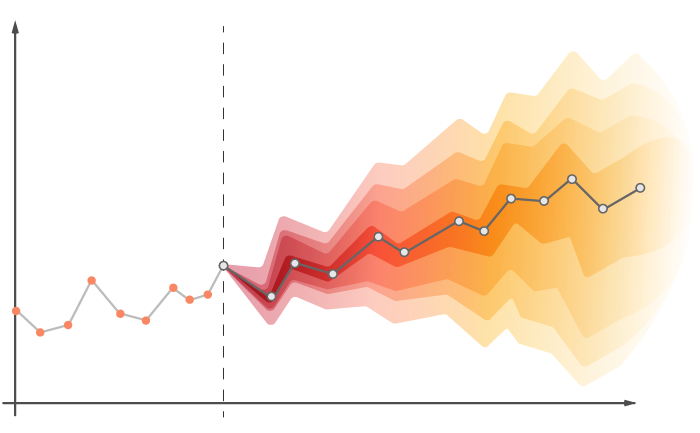
\includegraphics[height=1.5in]{./Images/probabilistic-forecasting-graph.png} \vspace{1in}
}

% Vanderbilt color scheme
\usepackage{xcolor}
\definecolor{gold}{RGB}{207,174,112}  % gold
\definecolor{black}{RGB}{10,10,10} % black
\definecolor{white}{RGB}{255,255,255} % white
\setbeamercolor{title}{fg = gold}
\setbeamercolor{title}{bg = black}
\setbeamercolor{normal text}{fg = black}
\setbeamercolor{frametitle}{fg = gold}
\setbeamercolor{frametitle}{bg = black}
\setbeamercolor{structure}{fg = gold}
\setbeamercolor{structure}{bg = black}
\setbeamercolor{item}{fg = black}

% Other stuff
\usepackage{amssymb}
\usepackage{ragged2e}
\usepackage{multicol}
\usepackage{mwe}

% Default setup
\usepackage[sfdefault]{cabin}
\usepackage{hyperref}
%\hypersetup{
%  colorlinks = true,
%  allcolors = blue
%}
\usepackage{float, placeins}
\usepackage{booktabs}

% Additional packages
\usepackage[edges]{forest}

% tikz equation packages
\usepackage{tikz}
\usetikzlibrary{backgrounds}
\usetikzlibrary{tikzmark}
\usetikzlibrary{calc}
\usetikzlibrary{arrows,shapes,positioning,shadows,trees,mindmap}
\usetikzlibrary{arrows.meta}
\colorlet{linecol}{black!75}
\usepackage{xkcdcolors} % xkcd colors

% Basic equation packages
\usepackage{amsmath}
\usepackage{amsthm}
\usepackage{amssymb}
\usepackage{mathtools}
\usepackage{nccmath}
\usepackage{wrapfig}
\usepackage{comment}
\usepackage{blindtext}
\usepackage{graphicx}
\usepackage{xspace}
\usepackage{array}
\usepackage{ragged2e}
\newcolumntype{P}[1]{>{\RaggedRight\hspace{0pt}}p{#1}}
\newcolumntype{X}[1]{>{\RaggedRight\hspace*{0pt}}p{#1}}
\DeclarePairedDelimiter{\norm}{\lVert}{\rVert}


% Color packages
\usepackage{xcolor}
\usepackage{tcolorbox}
\newcommand{\highlight}[2]{\colorbox{#1!30}{$\displaystyle #2$}}
\newcommand{\highlightdark}[2]{\colorbox{#1!50}{$\displaystyle #2$}}
\renewcommand{\highlight}[2]{\colorbox{#1!30}{#2}}
\renewcommand{\highlightdark}[2]{\colorbox{#1!50}{#2}}

% Define colors
\definecolor{red}{HTML}{F03D2D}
\definecolor{skyblue}{HTML}{90DDF0}
\definecolor{green}{HTML}{C8D96F}
\definecolor{orange}{HTML}{EF8A17}
\definecolor{yellow}{HTML}{F5C900}
\definecolor{purple}{HTML}{BA42C0}
\definecolor{teal}{HTML}{17BEBB}
\definecolor{greyblue}{HTML}{9BAFD9}

\ifLuaTeX
  \usepackage{selnolig}  % disable illegal ligatures
\fi

\title{Time Series Regression Models}
\author{DS-5740 Advanced Statistics}
\date{}

\begin{document}
\frame{\titlepage}

\begin{frame}{Overview}
\protect\hypertarget{overview}{}
\center Overview: Week 2
\end{frame}

\begin{frame}{Overview \textbar{} \small Week 2}
\protect\hypertarget{overview-week-2}{}
\textbf{Preliminaries}

\begin{itemize}
\item
  Quick coverage of important syllabus details \newline
\item
  Project 1 rubric \newline
\end{itemize}

\textbf{Goals for the Week}

\begin{itemize}
\item
  Consider factors involved in forecasting \newline
\item
  Make your first forecast and see forecasts \newline
\item
  Cover linear regression models with time series \newline
\item
  Make forecasts and check their accuracy
\end{itemize}
\end{frame}

\begin{frame}{Overview \textbar{} \small Week 2}
\protect\hypertarget{overview-week-2-1}{}
\textbf{Syllabus}

\begin{itemize}
\item
  Office Hours:

  \begin{itemize}
  \tightlist
  \item
    Alex: Tuesdays 2-3pm (Hobbs Building, Room 221); by appointment
    \newline
  \item
    Marisa: Thursdays 1-2pm (Sony Building, Room 2062) \newline
  \end{itemize}
\item
  Assignments:

  \begin{itemize}
  \tightlist
  \item
    Due on Sundays at midnight (.Rmd or .html over Brightspace) \newline
  \item
    Late work policy: can be turned in any time there after for 80\% of
    grade (until 11.20.2022) \newline
  \item
    12 assignments but only your \textit{10} highest grades count
  \end{itemize}
\end{itemize}

\textbf{Project 1 Rubric}
\end{frame}

\begin{frame}{Forecasting \textbar{} \small The Basics}
\protect\hypertarget{forecasting-the-basics}{}
\centering

What can we forecast?
\end{frame}

\begin{frame}{Difficulty of Forecasts}
\protect\hypertarget{difficulty-of-forecasts}{}
\begin{itemize}
\tightlist
\item
  daily electricity demand in three days \newline
\item
  time of sunrise this day next year \newline
\item
  Google stock price in 6 months (USD) \newline
\item
  maximum temperature tomorrow \newline
\item
  next week's gas prices (USD)
\end{itemize}
\end{frame}

\begin{frame}{Difficulty of Forecasts}
\protect\hypertarget{difficulty-of-forecasts-1}{}
\begin{enumerate}
\tightlist
\item
  time of sunrise this day next year \newline
\item
  maximum temperature tomorrow \newline
\item
  daily electricity demand in three days \newline
\item
  next week's gas prices (USD) \newline
\item
  Google stock price in 6 months (USD)
\end{enumerate}
\end{frame}

\begin{frame}{Factors Affecting Difficulty}
\protect\hypertarget{factors-affecting-difficulty}{}
\begin{enumerate}
\tightlist
\item
  knowledge of variables involved \newline
\item
  how much data are available \newline
\item
  similarity of future to past \newline
\item
  whether forecasts are useful
\end{enumerate}
\end{frame}

\begin{frame}{Consideration of Factors}
\protect\hypertarget{consideration-of-factors}{}
\begin{enumerate}
\tightlist
\item
  time of sunrise this day next year \newline \pause
\item
  maximum temperature tomorrow \newline \pause
\item
  daily electricity demand in three days \newline \pause
\item
  next week's gas prices (USD) \newline \pause
\item
  Google stock price in 6 months (USD)
\end{enumerate}
\end{frame}

\begin{frame}{Make a Forecast}
\protect\hypertarget{make-a-forecast}{}
\center Your Chance to Forecast
\end{frame}

\begin{frame}{Make a Forecast \textbar{} \small Plot Time Series}
\protect\hypertarget{make-a-forecast-plot-time-series}{}
\textbf{forecast}: an estimate of the probabilities of possible futures

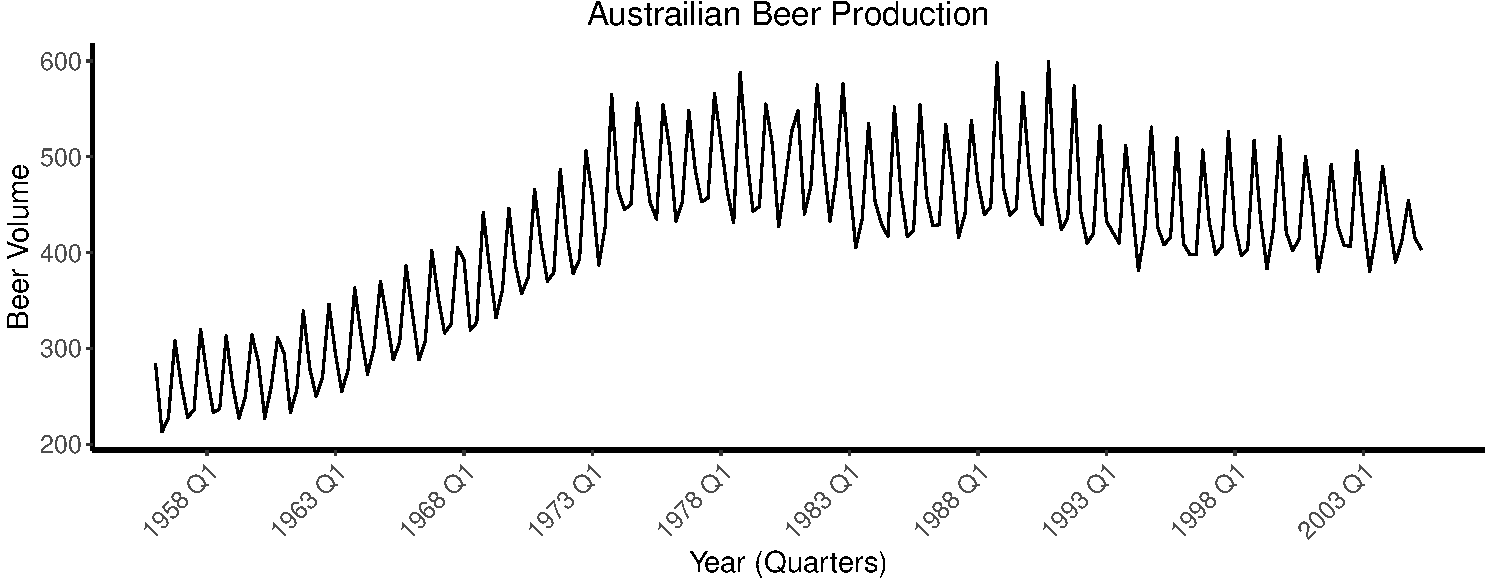
\includegraphics{Time-series-regression-models_files/figure-beamer/unnamed-chunk-3-1.pdf}
\end{frame}

\begin{frame}{Make a Forecast \textbar{} \small Basics}
\protect\hypertarget{make-a-forecast-basics}{}
\begin{enumerate}
\tightlist
\item
  Problem definition \newline
\item
  Gathering information \newline
\item
  Preliminary (exploratory) analysis \newline
\item
  Choosing and fitting models \newline
\item
  Using and evaluating a forecasting model
\end{enumerate}
\end{frame}

\begin{frame}{Make a Forecast \textbar{} \small Class Forecast}
\protect\hypertarget{make-a-forecast-class-forecast}{}
\textbf{forecast}: an estimate of the probabilities of possible futures

\vpsace{2cm}

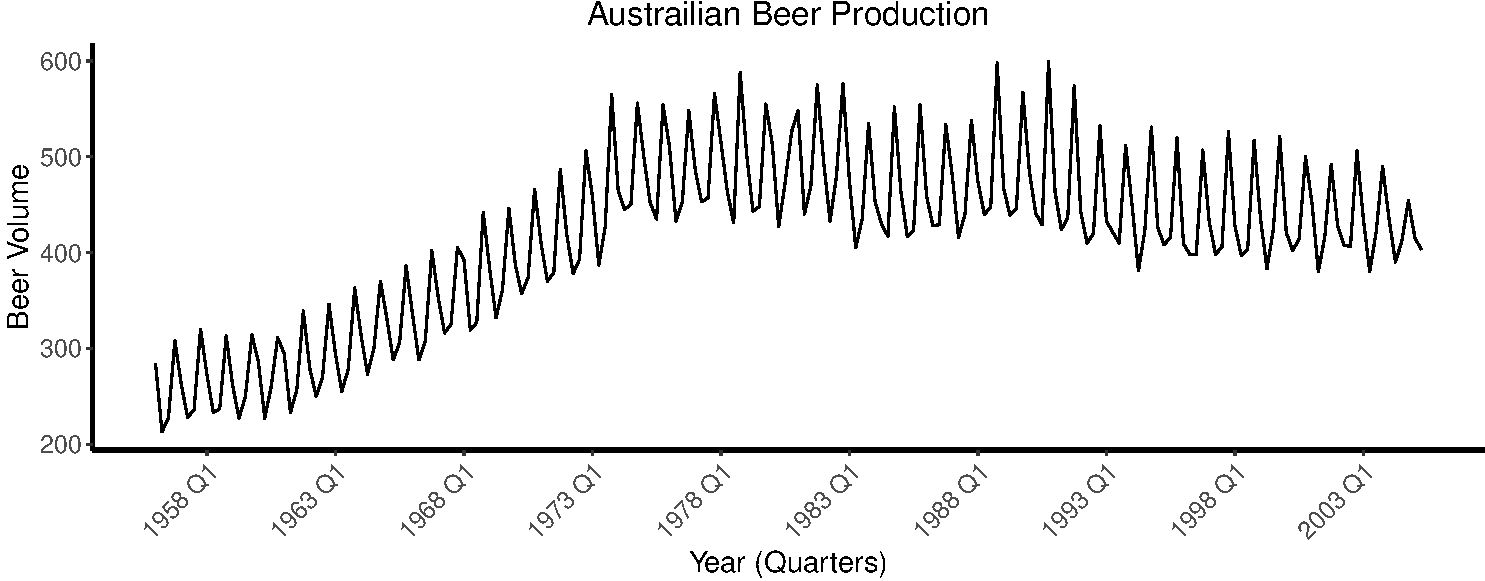
\includegraphics{Time-series-regression-models_files/figure-beamer/unnamed-chunk-4-1.pdf}
\end{frame}

\begin{frame}{Make a Forecast \textbar{} \small One Random Future}
\protect\hypertarget{make-a-forecast-one-random-future}{}
\textbf{forecast}: an estimate of the probabilities of possible futures

\vpsace{2cm}

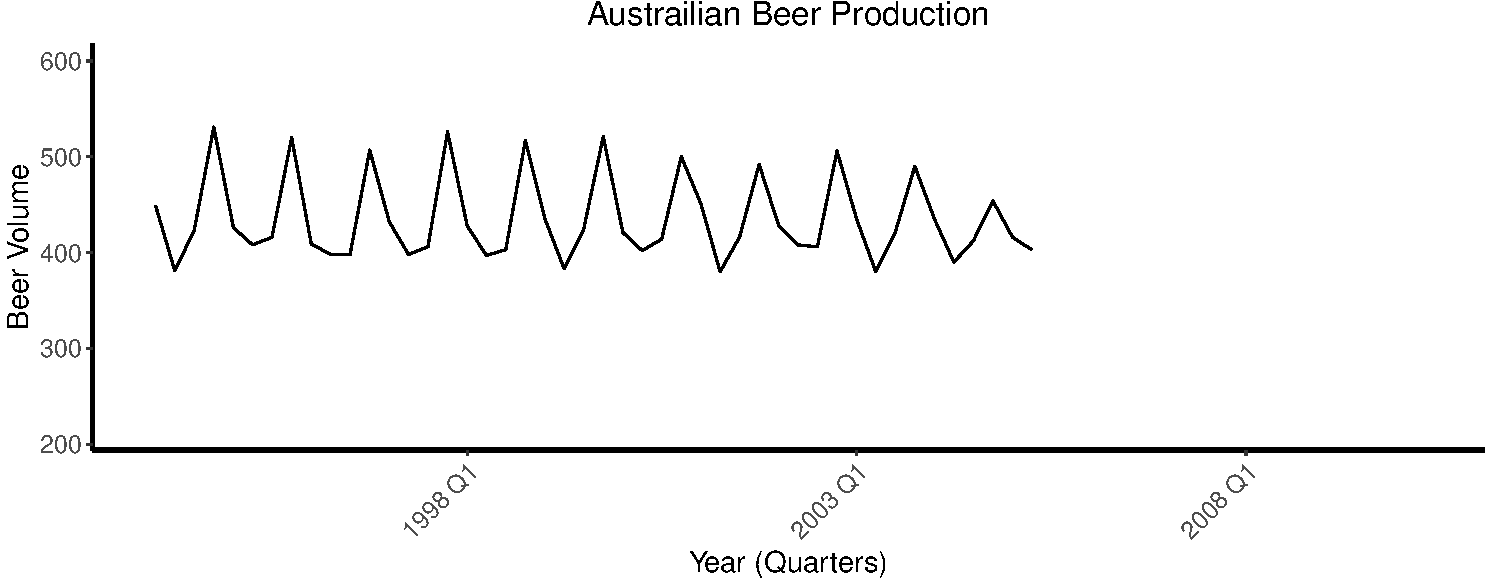
\includegraphics{Time-series-regression-models_files/figure-beamer/unnamed-chunk-5-1.pdf}
\end{frame}

\begin{frame}{Make a Forecast \textbar{} \small Ten Random Futures}
\protect\hypertarget{make-a-forecast-ten-random-futures}{}
\textbf{forecast}: an estimate of the probabilities of possible futures

\vpsace{2cm}

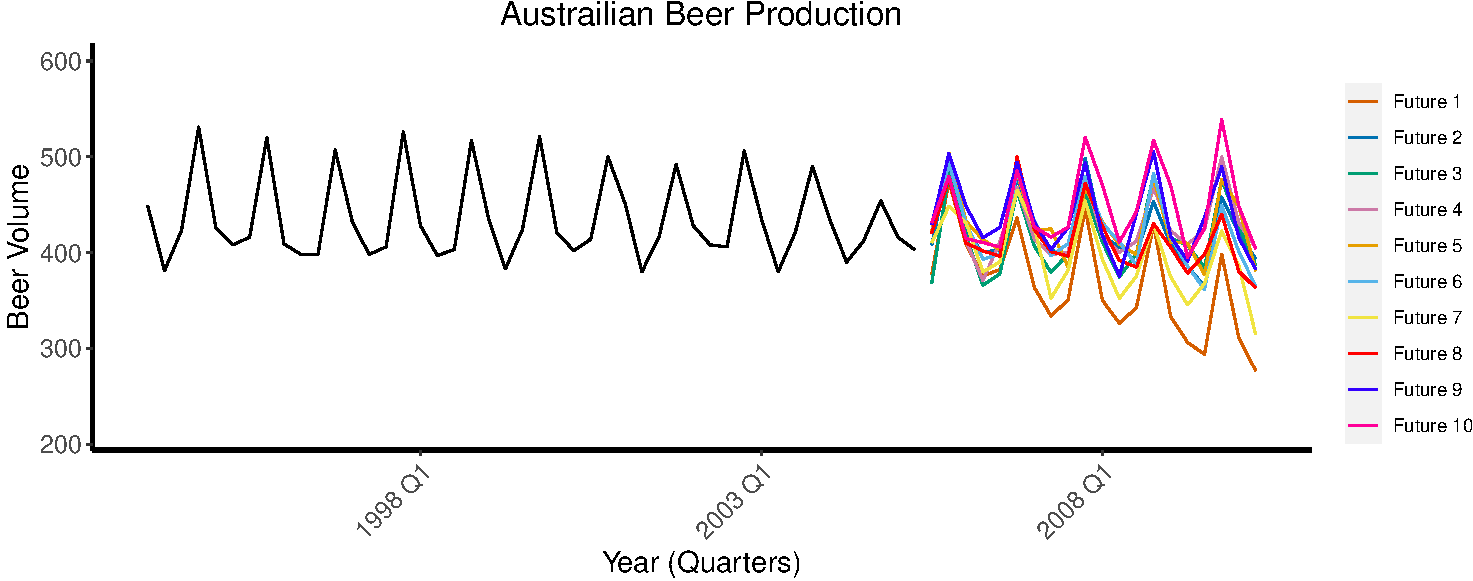
\includegraphics{Time-series-regression-models_files/figure-beamer/unnamed-chunk-6-1.pdf}
\end{frame}

\begin{frame}{Make a Forecast \textbar{} \small Actual Forecast}
\protect\hypertarget{make-a-forecast-actual-forecast}{}
\textbf{forecast}: an estimate of the probabilities of possible futures

\vpsace{2cm}

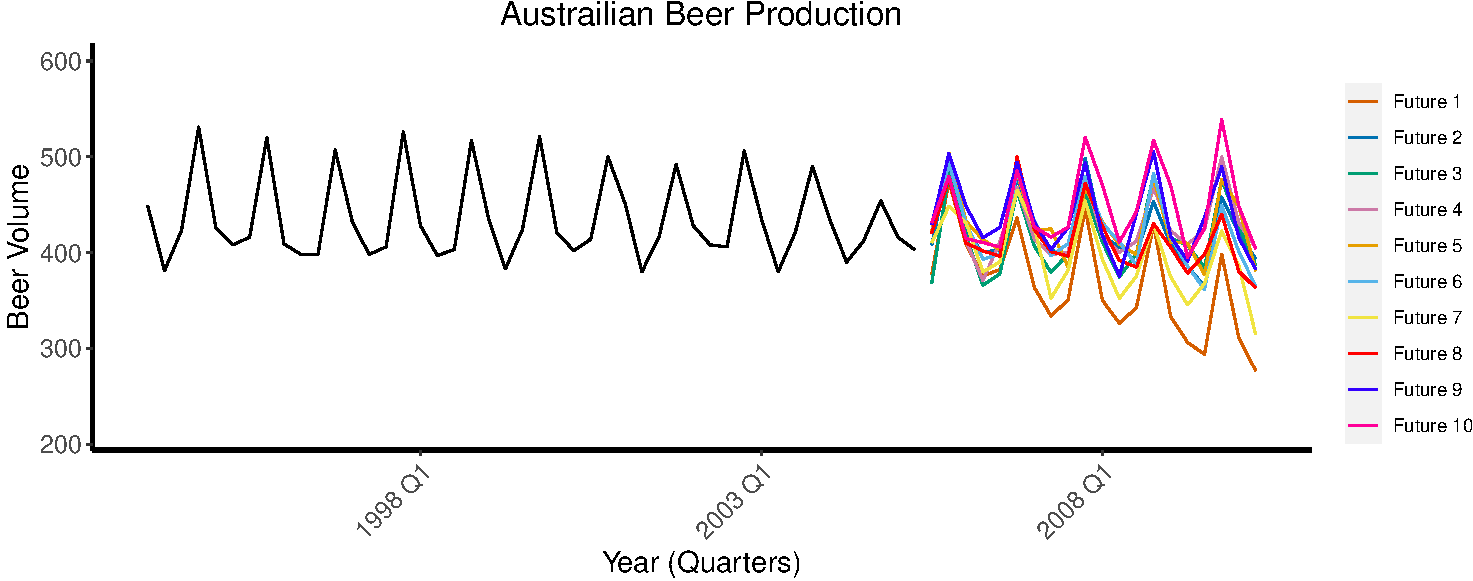
\includegraphics{Time-series-regression-models_files/figure-beamer/unnamed-chunk-7-1.pdf}
\end{frame}

\begin{frame}{Make a Forecast \textbar{} \small Ground Truth}
\protect\hypertarget{make-a-forecast-ground-truth}{}
\textbf{forecast}: an estimate of the probabilities of possible futures

\vpsace{2cm}

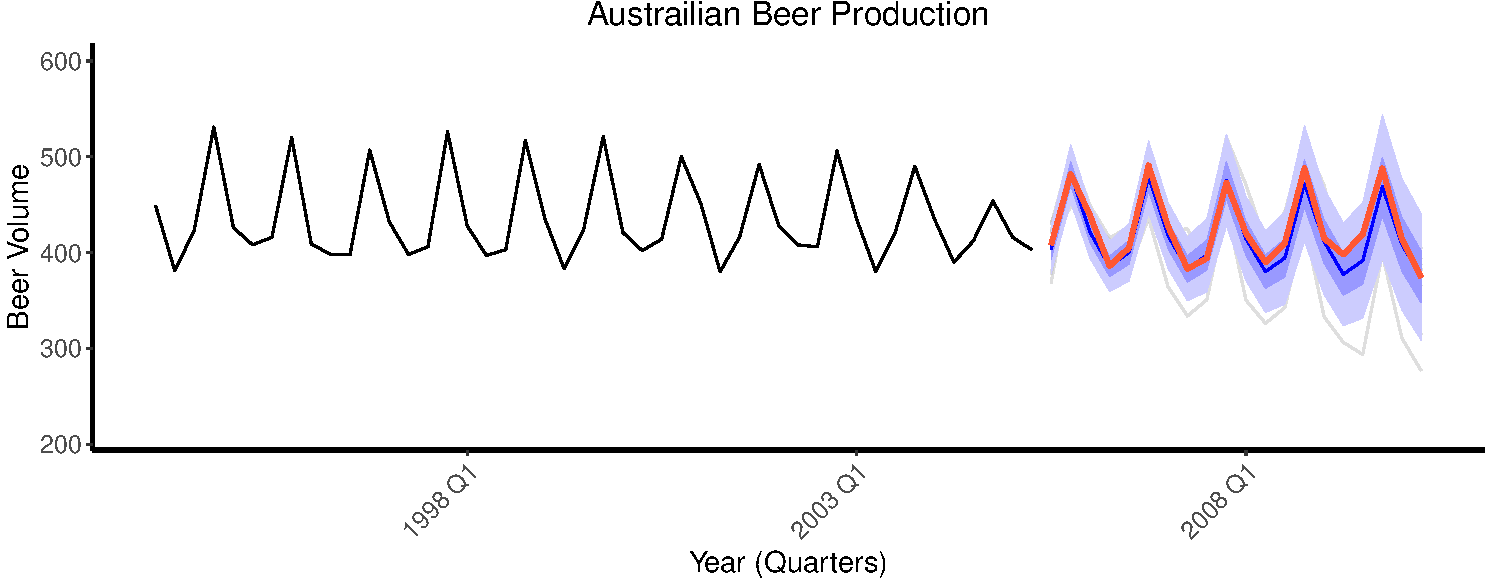
\includegraphics{Time-series-regression-models_files/figure-beamer/unnamed-chunk-8-1.pdf}
\end{frame}

\begin{frame}{Forecasting \textbar{} \small Regression}
\protect\hypertarget{forecasting-regression}{}
\center Times Series Linear Model (TSLM)
\end{frame}

\begin{frame}{Forecasting \textbar{} \small Regression}
\protect\hypertarget{forecasting-regression-1}{}
\[
y = \beta_0 + \sum_k^n \beta_k x_k + \epsilon
\]
\end{frame}

\begin{frame}{Forecasting \textbar{} \small Regression}
\protect\hypertarget{forecasting-regression-2}{}
\begin{figure}
\begin{equation*}
\tikzmarknode{y}{\highlight{red}{$y$}} =
\tikzmarknode{intercept}{\highlight{skyblue}{$\beta_0$}} +
\tikzmarknode{betas}{\highlight{green}{$\sum_k^n \beta_k x_k$}} +
\tikzmarknode{error}{\highlight{orange}{$\epsilon$}}
\end{equation*}

\begin{tikzpicture}[overlay,remember picture,>=stealth,nodes={align=center,inner ysep=1pt},<-]
    
    % y
    \path (y.north) ++ (0,1em) node[anchor=south east,color=red] (scalep){\textbf{outcome}};
    \draw [color=red](y.north) |- ([xshift=-0.3ex,color=red]scalep.south west);
    
    % intercept
    \path (intercept.south) ++ (0,-1em) node[anchor=north east,color=skyblue] (scalep){\textbf{intercept}};
    \draw [color=skyblue](intercept.south) |- ([xshift=-0.3ex,color=skyblue]scalep.north west);
    
    % betas
    \path (betas.north) ++ (0,1em) node[anchor=south west,color=green] (scalep){\textbf{sum of weights by predictor}};
    \draw [color=green](betas.north) |- ([xshift=-0.3ex,color=green]scalep.south east);
    
    % error
    \path (error.south) ++ (0,-1em) node[anchor=north west,color=orange] (scalep){\textbf{error}};
    \draw [color=orange](error.south) |- ([xshift=-0.3ex,color=orange]scalep.north east);
    
\end{tikzpicture}
\vspace{-1.1cm}
\label{fig:fig1}
\end{figure}
\end{frame}

\begin{frame}{Forecasting \textbar{} \small Regression}
\protect\hypertarget{forecasting-regression-3}{}
\centering
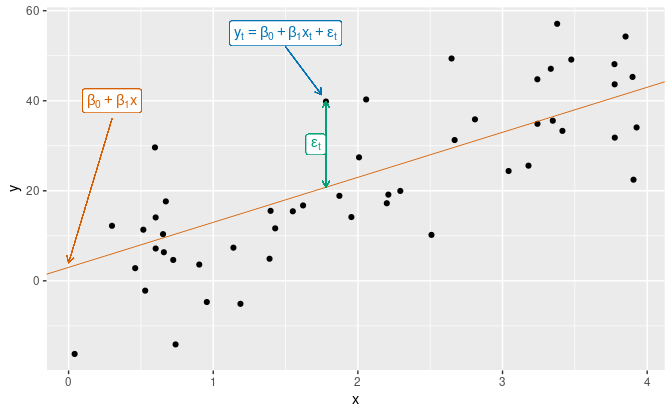
\includegraphics[height=2.5in]{./Images/linear-regression.png}
\end{frame}

\begin{frame}{Forecasting \textbar{} \small Regression with Time}
\protect\hypertarget{forecasting-regression-with-time}{}
\[
y_t = \beta_0 + \sum_k^n \beta_k x_{k, t} + \epsilon_t
\]
\end{frame}

\begin{frame}{Forecasting \textbar{} \small Regression with Time}
\protect\hypertarget{forecasting-regression-with-time-1}{}
\begin{figure}
\begin{equation*}
\tikzmarknode{y}{\highlight{red}{$y_t$}} =
\tikzmarknode{intercept}{\highlight{skyblue}{$\beta_0$}} +
\tikzmarknode{betas}{\highlight{green}{$\sum_k^n \beta_k x_{k, t}$}} +
\tikzmarknode{error}{\highlight{orange}{$\epsilon_t$}}
\end{equation*}

\begin{tikzpicture}[overlay,remember picture,>=stealth,nodes={align=center,inner ysep=1pt},<-]
    
    % y
    \path (y.north) ++ (0,1em) node[anchor=south east,color=red] (scalep){\textbf{outcome (at time \textit{t})}};
    \draw [color=red](y.north) |- ([xshift=-0.3ex,color=red]scalep.south west);
    
    % intercept
    \path (intercept.south) ++ (0,-1em) node[anchor=north east,color=skyblue] (scalep){\textbf{intercept}};
    \draw [color=skyblue](intercept.south) |- ([xshift=-0.3ex,color=skyblue]scalep.north west);
    
    % betas
    \path (betas.north) ++ (0,1em) node[anchor=south west,color=green] (scalep){\textbf{sum of weights by predictor} \\ \textbf{(at time \textit{t})}};
    \draw [color=green](betas.north) |- ([xshift=-0.3ex,color=green]scalep.south east);
    
    % error
    \path (error.south) ++ (0,-1em) node[anchor=north west,color=orange] (scalep){\textbf{error (at time \textit{t})}};
    \draw [color=orange](error.south) |- ([xshift=-0.3ex,color=orange]scalep.north east);
    
\end{tikzpicture}
\vspace{-1.1cm}
\label{fig:fig2}
\end{figure}

\vspace{1cm}

\pause

\begin{itemize}
\tightlist
\item
  \(y_t\) = \textbf{outcome} or variable we want to predict
\end{itemize}

\pause

\begin{itemize}
\item
  \(x_k,t\) = \textbf{predictor} or variable used to predict the outcome

  \begin{itemize}
  \tightlist
  \item
    Usually assumed to be known for all \textit{past} and
    \textit{future}
  \end{itemize}
\end{itemize}

\pause

\begin{itemize}
\tightlist
\item
  \(\beta_k\) = \textbf{coefficients} that measure the effect of each
  predictor (after taking into account all other predictors)
\end{itemize}

\pause

\begin{itemize}
\tightlist
\item
  \(\epsilon_t\) = white noise error term (we'll talk more on this
  later)
\end{itemize}
\end{frame}

\begin{frame}{Forecasting \textbar{} \small Regression Example}
\protect\hypertarget{forecasting-regression-example}{}
\center Regression Example
\end{frame}

\begin{frame}{Forecasting \textbar{} \small US Consumption Expediture}
\protect\hypertarget{forecasting-us-consumption-expediture}{}
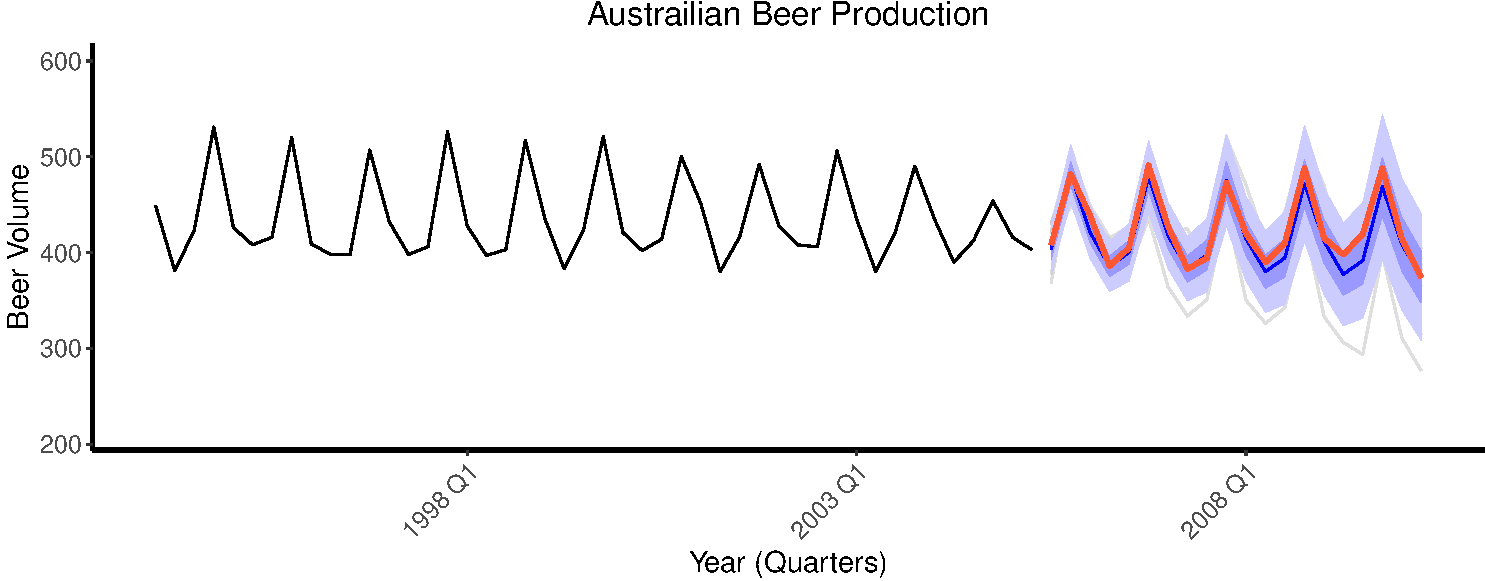
\includegraphics{Time-series-regression-models_files/figure-beamer/unnamed-chunk-9-1.pdf}
\end{frame}

\begin{frame}{Forecasting \textbar{} \small US Consumption Expediture}
\protect\hypertarget{forecasting-us-consumption-expediture-1}{}
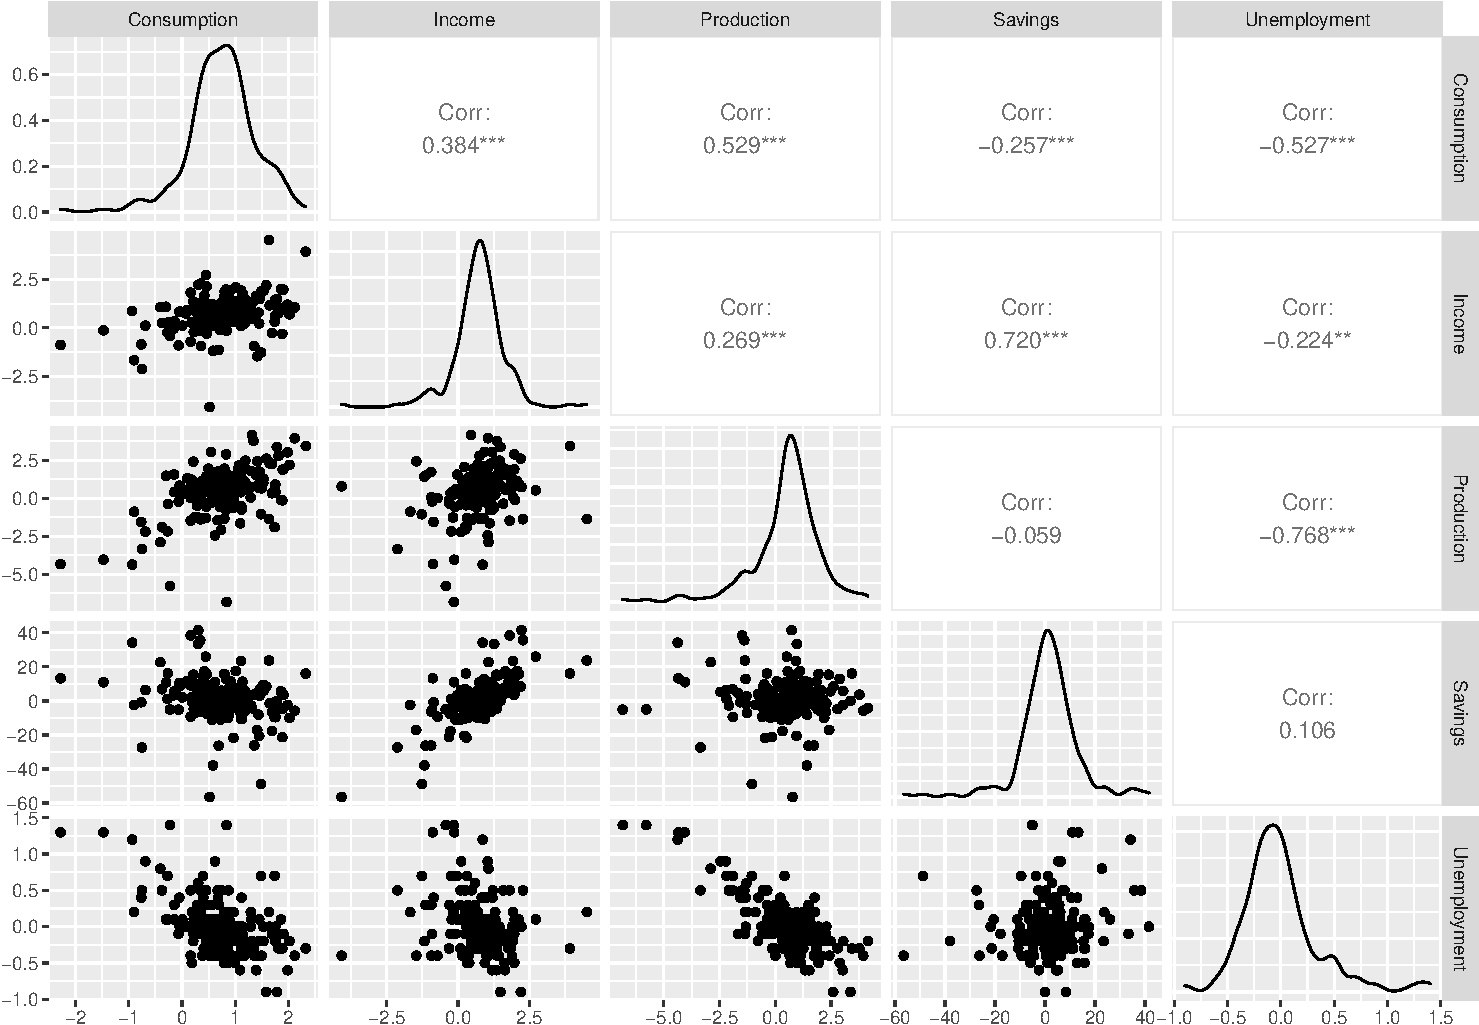
\includegraphics{Time-series-regression-models_files/figure-beamer/unnamed-chunk-10-1.pdf}
\end{frame}

\begin{frame}[fragile]{Forecasting \textbar{} \small US Consumption
Expediture}
\protect\hypertarget{forecasting-us-consumption-expediture-2}{}
\footnotesize

\normalfont

\footnotesize

\begin{verbatim}
Series: Consumption 
Model: TSLM 

Residuals:
     Min       1Q   Median       3Q      Max 
-0.90555 -0.15821 -0.03608  0.13618  1.15471 

Coefficients:
              Estimate Std. Error t value Pr(>|t|)    
(Intercept)   0.253105   0.034470   7.343 5.71e-12 ***
Income        0.740583   0.040115  18.461  < 2e-16 ***
Production    0.047173   0.023142   2.038   0.0429 *  
Unemployment -0.174685   0.095511  -1.829   0.0689 .  
Savings      -0.052890   0.002924 -18.088  < 2e-16 ***
---
Signif. codes:  0 '***' 0.001 '**' 0.01 '*' 0.05 '.' 0.1 ' ' 1

Residual standard error: 0.3102 on 193 degrees of freedom
Multiple R-squared: 0.7683, Adjusted R-squared: 0.7635
F-statistic:   160 on 4 and 193 DF, p-value: < 2.22e-16
\end{verbatim}

\normalfont
\end{frame}

\begin{frame}[fragile]{Forecasting \textbar{} \small Regression Example}
\protect\hypertarget{forecasting-regression-example-1}{}
\footnotesize

\normalfont

\footnotesize

\begin{Shaded}
\begin{Highlighting}[]
\CommentTok{\# Load \{fpp3\}}
\FunctionTok{library}\NormalTok{(fpp3)}

\CommentTok{\# Load US Consumption data}
\FunctionTok{data}\NormalTok{(}\StringTok{"us\_change"}\NormalTok{)}

\CommentTok{\# Length of time series}
\NormalTok{ts\_length }\OtherTok{\textless{}{-}} \FunctionTok{nrow}\NormalTok{(us\_change)}

\CommentTok{\# Remove last five years (we\textquotesingle{}ll make a prediction later) }
\NormalTok{us\_prediction }\OtherTok{\textless{}{-}}\NormalTok{ us\_change[}
  \SpecialCharTok{{-}}\FunctionTok{c}\NormalTok{((ts\_length }\SpecialCharTok{{-}} \DecValTok{19}\NormalTok{)}\SpecialCharTok{:}\NormalTok{ts\_length), }\CommentTok{\# remove last 5 years}
\NormalTok{]}

\CommentTok{\# Save last five years (we\textquotesingle{}ll compare with prediction)}
\NormalTok{us\_actual }\OtherTok{\textless{}{-}}\NormalTok{ us\_change[}
  \FunctionTok{c}\NormalTok{((ts\_length }\SpecialCharTok{{-}} \DecValTok{19}\NormalTok{)}\SpecialCharTok{:}\NormalTok{ts\_length), }\CommentTok{\# keeps last 5 years}
\NormalTok{]}
\end{Highlighting}
\end{Shaded}

\normalfont
\end{frame}

\begin{frame}[fragile]{Forecasting \textbar{} \small Regression Example}
\protect\hypertarget{forecasting-regression-example-2}{}
\footnotesize

\begin{Shaded}
\begin{Highlighting}[]
\CommentTok{\# Fit linear model}
\NormalTok{fit\_us\_lm }\OtherTok{\textless{}{-}}\NormalTok{ us\_prediction }\SpecialCharTok{\%\textgreater{}\%} \CommentTok{\# our data}
  \FunctionTok{model}\NormalTok{( }\CommentTok{\# model for time series}
    \AttributeTok{tslm =} \FunctionTok{TSLM}\NormalTok{( }\CommentTok{\# time series linear model}
\NormalTok{      Consumption }\SpecialCharTok{\textasciitilde{}}\NormalTok{ Income }\SpecialCharTok{+}\NormalTok{ Production }\SpecialCharTok{+}\NormalTok{ Savings }\SpecialCharTok{+}\NormalTok{ Unemployment}
\NormalTok{    )}
\NormalTok{  )}
\end{Highlighting}
\end{Shaded}

\normalfont
\end{frame}

\begin{frame}[fragile]{Forecasting \textbar{} \small Regression Example}
\protect\hypertarget{forecasting-regression-example-3}{}
\tiny

\normalfont

\tiny

\begin{Shaded}
\begin{Highlighting}[]
\CommentTok{\# Report fit}
\FunctionTok{report}\NormalTok{(fit\_us\_lm)}
\end{Highlighting}
\end{Shaded}

\begin{verbatim}
Series: Consumption 
Model: TSLM 

Residuals:
     Min       1Q   Median       3Q      Max 
-0.89952 -0.16879 -0.03979  0.13944  1.14909 

Coefficients:
              Estimate Std. Error t value Pr(>|t|)    
(Intercept)   0.261795   0.037847   6.917 8.56e-11 ***
Income        0.737779   0.042300  17.442  < 2e-16 ***
Production    0.044788   0.026403   1.696   0.0916 .  
Savings      -0.052416   0.003091 -16.960  < 2e-16 ***
Unemployment -0.191468   0.107811  -1.776   0.0775 .  
---
Signif. codes:  0 '***' 0.001 '**' 0.01 '*' 0.05 '.' 0.1 ' ' 1

Residual standard error: 0.3251 on 173 degrees of freedom
Multiple R-squared: 0.768,  Adjusted R-squared: 0.7627
F-statistic: 143.2 on 4 and 173 DF, p-value: < 2.22e-16
\end{verbatim}

\normalfont
\end{frame}

\begin{frame}{Forecasting \textbar{} \small Regression Example}
\protect\hypertarget{forecasting-regression-example-4}{}
\center Forecasting with Regression
\end{frame}

\begin{frame}[fragile]{Forecasting \textbar{} \small Regression Example}
\protect\hypertarget{forecasting-regression-example-5}{}
\tiny

\normalfont

\tiny

\begin{Shaded}
\begin{Highlighting}[]
\CommentTok{\# Plot model}
\FunctionTok{augment}\NormalTok{(fit\_us\_lm) }\SpecialCharTok{\%\textgreater{}\%}
  \CommentTok{\# Plot quarter on x{-}axis}
  \FunctionTok{ggplot}\NormalTok{(}\FunctionTok{aes}\NormalTok{(}\AttributeTok{x =}\NormalTok{ Quarter)) }\SpecialCharTok{+}
  \CommentTok{\# Plot actual values}
  \FunctionTok{geom\_line}\NormalTok{(}\FunctionTok{aes}\NormalTok{(}\AttributeTok{y =}\NormalTok{ Consumption, }\AttributeTok{colour =} \StringTok{"Data"}\NormalTok{)) }\SpecialCharTok{+}
  \CommentTok{\# Plot fit values}
  \FunctionTok{geom\_line}\NormalTok{(}\FunctionTok{aes}\NormalTok{(}\AttributeTok{y =}\NormalTok{ .fitted, }\AttributeTok{colour =} \StringTok{"Fitted"}\NormalTok{)) }\SpecialCharTok{+}
  \FunctionTok{labs}\NormalTok{(}
    \CommentTok{\# No y{-}axis label}
    \AttributeTok{y =} \ConstantTok{NULL}\NormalTok{, }
    \CommentTok{\# Change title}
    \AttributeTok{title =} \StringTok{"Percent change in US consumption expenditure"}
\NormalTok{  ) }\SpecialCharTok{+}
  \CommentTok{\# Change colors}
  \FunctionTok{scale\_colour\_manual}\NormalTok{(}
    \AttributeTok{values =} \FunctionTok{c}\NormalTok{(}
      \AttributeTok{Data =} \StringTok{"black"}\NormalTok{, }\CommentTok{\# Make data line black}
      \AttributeTok{Fitted =} \StringTok{"orange"} \CommentTok{\# Make fitted line orange}
\NormalTok{    )}
\NormalTok{  ) }\SpecialCharTok{+}
  \CommentTok{\# No title for legend}
  \FunctionTok{guides}\NormalTok{(}\AttributeTok{colour =} \FunctionTok{guide\_legend}\NormalTok{(}\AttributeTok{title =} \ConstantTok{NULL}\NormalTok{))}
\end{Highlighting}
\end{Shaded}

\normalfont
\end{frame}

\begin{frame}{Forecasting \textbar{} \small Regression Example}
\protect\hypertarget{forecasting-regression-example-6}{}
\tiny

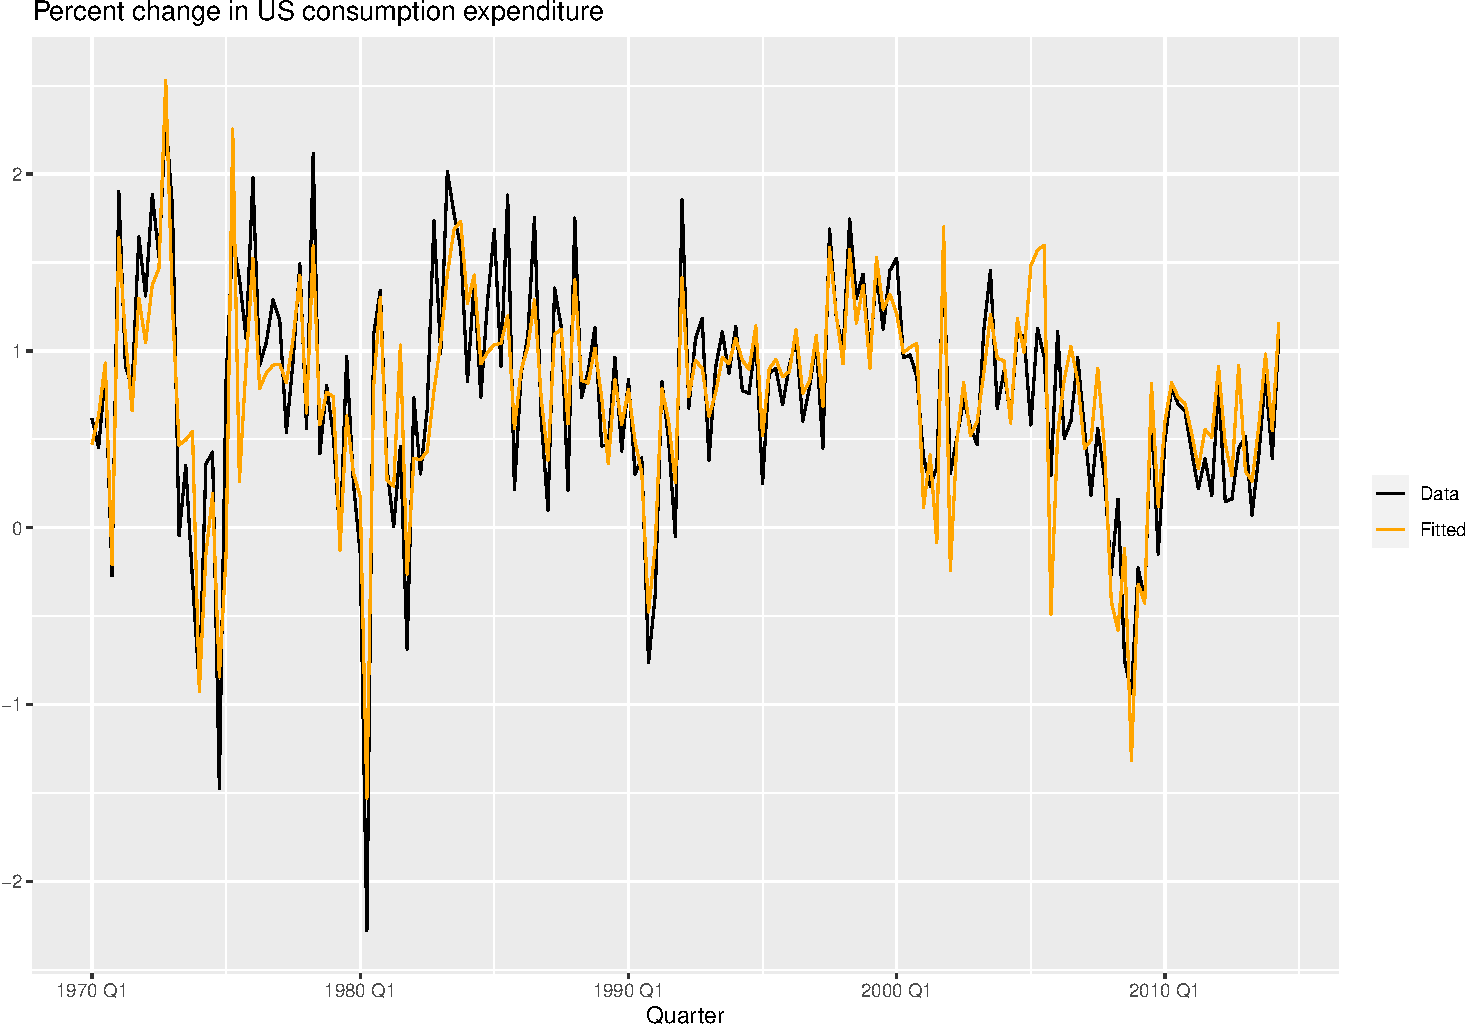
\includegraphics{Time-series-regression-models_files/figure-beamer/unnamed-chunk-20-1.pdf}

\normalfont
\end{frame}

\begin{frame}[fragile]{Forecasting \textbar{} \small Regression
Forecast}
\protect\hypertarget{forecasting-regression-forecast}{}
\tiny

\begin{Shaded}
\begin{Highlighting}[]
\CommentTok{\# Forecast}
\NormalTok{fc }\OtherTok{\textless{}{-}} \FunctionTok{forecast}\NormalTok{(fit\_us\_lm, }\AttributeTok{new\_data =}\NormalTok{ us\_actual)}

\CommentTok{\# Plot forecast}
\NormalTok{us\_change }\SpecialCharTok{\%\textgreater{}\%}
  \CommentTok{\# Plot quarter on x{-}axis}
  \FunctionTok{ggplot}\NormalTok{(}\FunctionTok{aes}\NormalTok{(}\AttributeTok{x =}\NormalTok{ Quarter)) }\SpecialCharTok{+}
  \CommentTok{\# Plot actual values}
  \FunctionTok{geom\_line}\NormalTok{(}\FunctionTok{aes}\NormalTok{(}\AttributeTok{y =}\NormalTok{ Consumption, }\AttributeTok{colour =} \StringTok{"Data"}\NormalTok{)) }\SpecialCharTok{+}
  \CommentTok{\# Plot predicted values}
  \FunctionTok{geom\_line}\NormalTok{(}
    \AttributeTok{data =}\NormalTok{ fc,}
    \FunctionTok{aes}\NormalTok{(}\AttributeTok{y =}\NormalTok{ .mean, }\AttributeTok{colour =} \StringTok{"Fitted"}\NormalTok{),}
    \AttributeTok{size =} \DecValTok{1}
\NormalTok{  ) }\SpecialCharTok{+}
  \FunctionTok{labs}\NormalTok{(}
    \CommentTok{\# No y{-}axis label}
    \AttributeTok{y =} \ConstantTok{NULL}\NormalTok{, }
    \CommentTok{\# Change title}
    \AttributeTok{title =} \StringTok{"Percent change in US consumption expenditure"}
\NormalTok{  ) }\SpecialCharTok{+}
  \CommentTok{\# Change colors}
  \FunctionTok{scale\_colour\_manual}\NormalTok{(}
    \AttributeTok{values =} \FunctionTok{c}\NormalTok{(}
      \AttributeTok{Data =} \StringTok{"black"}\NormalTok{, }\CommentTok{\# Make data line black}
      \AttributeTok{Fitted =} \StringTok{"orange"} \CommentTok{\# Make fitted line orange}
\NormalTok{    )}
\NormalTok{  ) }\SpecialCharTok{+}
  \CommentTok{\# No title for legend}
  \FunctionTok{guides}\NormalTok{(}\AttributeTok{colour =} \FunctionTok{guide\_legend}\NormalTok{(}\AttributeTok{title =} \ConstantTok{NULL}\NormalTok{))}
\end{Highlighting}
\end{Shaded}

\normalfont
\end{frame}

\begin{frame}{Forecasting \textbar{} \small Regression Forecast}
\protect\hypertarget{forecasting-regression-forecast-1}{}
\tiny

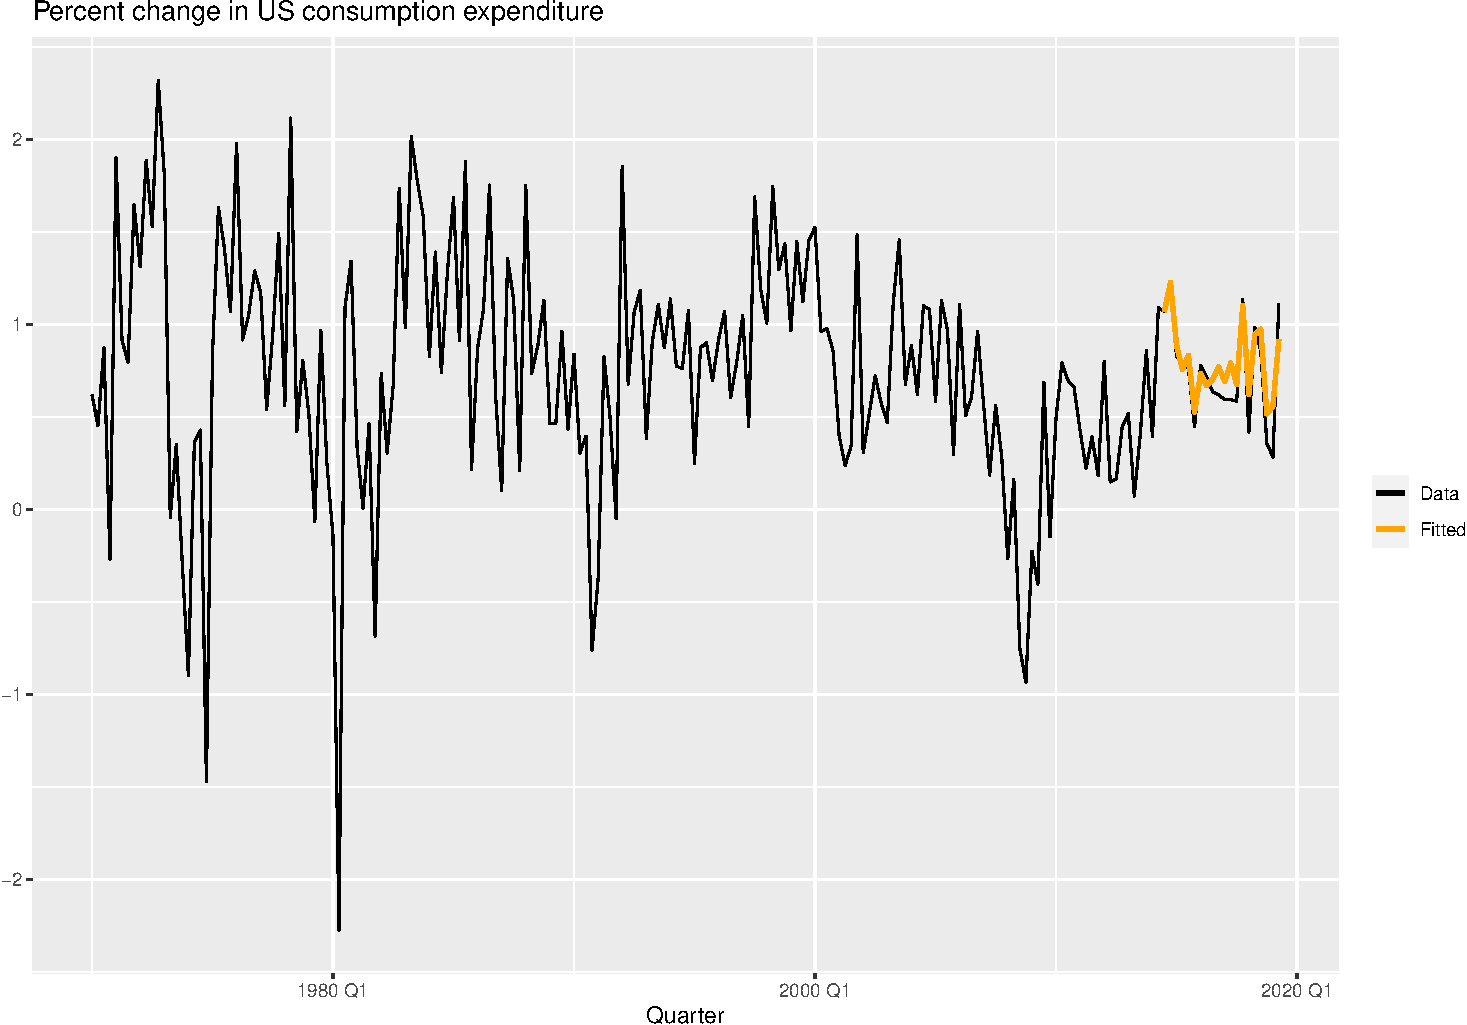
\includegraphics{Time-series-regression-models_files/figure-beamer/unnamed-chunk-22-1.pdf}

\normalfont
\end{frame}

\begin{frame}{Forecasting \textbar{} \small Regression Forecast
Accuracy}
\protect\hypertarget{forecasting-regression-forecast-accuracy}{}
\begin{block}{Measures of Accuracy}
\protect\hypertarget{measures-of-accuracy}{}
\begin{itemize}
\tightlist
\item
  R-squared: proportion of variance explained \newline
\end{itemize}

\center \(R^2 = \frac{\sum(\hat{y_t} - \bar{y})^2}{\sum(y_t - \bar{y})^2}\)
\newline

\begin{itemize}
\tightlist
\item
  Mean absolute error: average error \newline
\end{itemize}

\center \(MAE = \frac{\sum |\hat{y_t} - y_t|}{T}\) \newline

\begin{itemize}
\tightlist
\item
  Root mean square error: standard deviation of error \newline
\end{itemize}

\center \(RMSE = \sqrt{\frac{\sum (\hat{y_t} - y_t)^2}{T}}\) \newline

\begin{itemize}
\tightlist
\item
  Mean bias error: tendency to over- (+) or underestimate (-) \newline
\end{itemize}

\center \(MBE = \frac{\sum \hat{y_t} - y_t}{T}\)
\end{block}
\end{frame}

\begin{frame}[fragile]{Forecasting \textbar{} \small Regression Forecast
Accuracy}
\protect\hypertarget{forecasting-regression-forecast-accuracy-1}{}
\small

\normalfont

\small

\begin{Shaded}
\begin{Highlighting}[]
\CommentTok{\# R{-}squared}
\FunctionTok{cor}\NormalTok{(fc}\SpecialCharTok{$}\NormalTok{.mean, us\_actual}\SpecialCharTok{$}\NormalTok{Consumption)}\SpecialCharTok{\^{}}\DecValTok{2}
\end{Highlighting}
\end{Shaded}

\begin{verbatim}
[1] 0.8647245
\end{verbatim}

\begin{Shaded}
\begin{Highlighting}[]
\CommentTok{\# MAE}
\FunctionTok{mean}\NormalTok{(}\FunctionTok{abs}\NormalTok{(fc}\SpecialCharTok{$}\NormalTok{.mean }\SpecialCharTok{{-}}\NormalTok{ us\_actual}\SpecialCharTok{$}\NormalTok{Consumption))}
\end{Highlighting}
\end{Shaded}

\begin{verbatim}
[1] 0.1000182
\end{verbatim}

\begin{Shaded}
\begin{Highlighting}[]
\CommentTok{\# RMSE}
\FunctionTok{sqrt}\NormalTok{(}\FunctionTok{mean}\NormalTok{((fc}\SpecialCharTok{$}\NormalTok{.mean }\SpecialCharTok{{-}}\NormalTok{ us\_actual}\SpecialCharTok{$}\NormalTok{Consumption)}\SpecialCharTok{\^{}}\DecValTok{2}\NormalTok{))}
\end{Highlighting}
\end{Shaded}

\begin{verbatim}
[1] 0.1235474
\end{verbatim}

\begin{Shaded}
\begin{Highlighting}[]
\CommentTok{\# MBE}
\FunctionTok{mean}\NormalTok{(fc}\SpecialCharTok{$}\NormalTok{.mean }\SpecialCharTok{{-}}\NormalTok{ us\_actual}\SpecialCharTok{$}\NormalTok{Consumption)}
\end{Highlighting}
\end{Shaded}

\begin{verbatim}
[1] 0.06020543
\end{verbatim}

\normalfont
\end{frame}

\begin{frame}[fragile]{Forecasting \textbar{} \small Regression
Residuals}
\protect\hypertarget{forecasting-regression-residuals}{}
\footnotesize

\normalfont

\footnotesize

\begin{Shaded}
\begin{Highlighting}[]
\CommentTok{\# Check residuals}
\FunctionTok{gg\_tsresiduals}\NormalTok{(fit\_us\_lm)}
\end{Highlighting}
\end{Shaded}

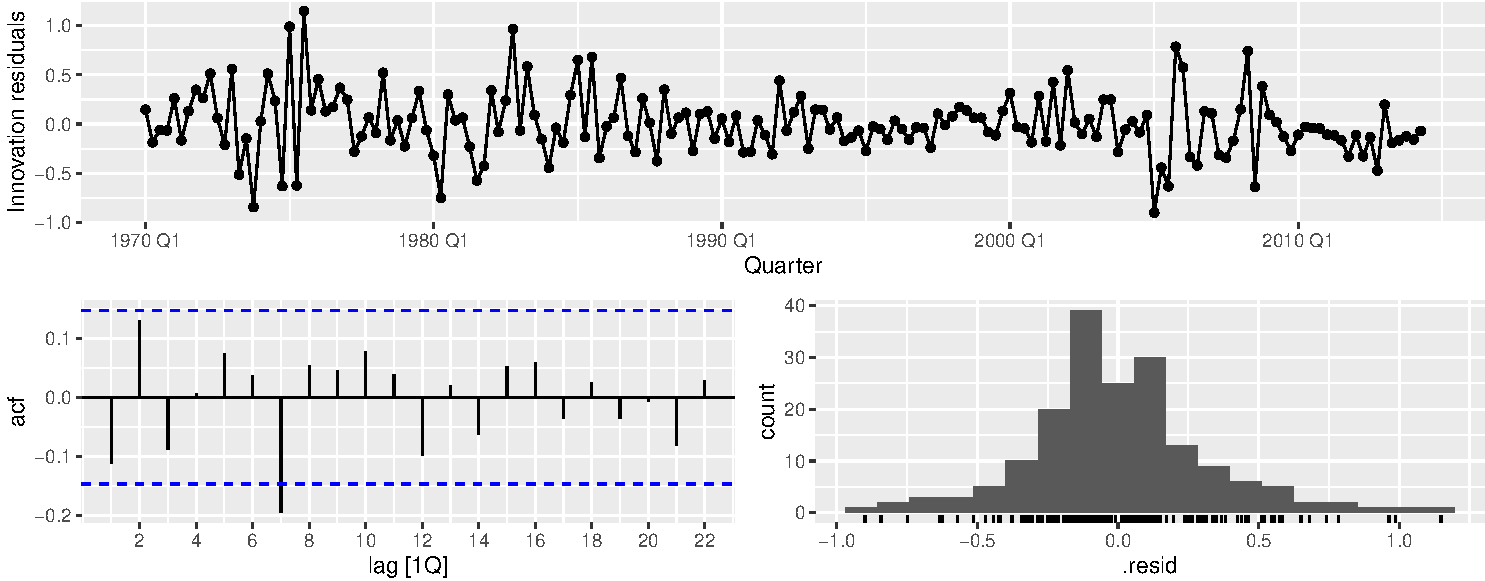
\includegraphics{Time-series-regression-models_files/figure-beamer/unnamed-chunk-26-1.pdf}

\normalfont
\end{frame}

\begin{frame}[fragile]{Forecasting \textbar{} \small Regression Forecast
(no actual data)}
\protect\hypertarget{forecasting-regression-forecast-no-actual-data}{}
\tiny

\normalfont

\tiny

\begin{Shaded}
\begin{Highlighting}[]
\CommentTok{\# Future scenarios}
\NormalTok{future\_scenarios }\OtherTok{\textless{}{-}} \FunctionTok{scenarios}\NormalTok{( }\CommentTok{\# Create future scenarios}
  \AttributeTok{increase\_income =} \FunctionTok{new\_data}\NormalTok{( }\CommentTok{\# Create new data}
\NormalTok{    us\_prediction,  }\CommentTok{\# Original data}
    \FunctionTok{nrow}\NormalTok{(us\_actual) }\CommentTok{\# Number of new data}
\NormalTok{  ) }\SpecialCharTok{\%\textgreater{}\%}
    \FunctionTok{mutate}\NormalTok{(}
      \AttributeTok{Income =} \FunctionTok{mean}\NormalTok{(us\_prediction}\SpecialCharTok{$}\NormalTok{Income) }\SpecialCharTok{+} \CommentTok{\# Add to mean Income}
        \FunctionTok{seq}\NormalTok{(}\DecValTok{0}\NormalTok{, }\DecValTok{1}\NormalTok{, }\AttributeTok{length =} \FunctionTok{nrow}\NormalTok{(us\_actual)), }\CommentTok{\# Increase from 0 to 1}
      \CommentTok{\# with a length equal to the number of actual data}
      \AttributeTok{Production =} \FunctionTok{mean}\NormalTok{(us\_prediction}\SpecialCharTok{$}\NormalTok{Production) }\SpecialCharTok{+} 
        \FunctionTok{rep}\NormalTok{(}\DecValTok{0}\NormalTok{, }\FunctionTok{nrow}\NormalTok{(us\_actual)), }\CommentTok{\# No increase/decrease}
      \CommentTok{\# Repeat 0 with a length equal to the number of actual data}
      \AttributeTok{Savings =} \FunctionTok{mean}\NormalTok{(us\_prediction}\SpecialCharTok{$}\NormalTok{Savings) }\SpecialCharTok{+} 
        \FunctionTok{rep}\NormalTok{(}\DecValTok{0}\NormalTok{, }\FunctionTok{nrow}\NormalTok{(us\_actual)),}
      \AttributeTok{Unemployment =} \FunctionTok{mean}\NormalTok{(us\_prediction}\SpecialCharTok{$}\NormalTok{Unemployment) }\SpecialCharTok{+}
        \FunctionTok{rep}\NormalTok{(}\DecValTok{0}\NormalTok{, }\FunctionTok{nrow}\NormalTok{(us\_actual))}
\NormalTok{    ),}
  \AttributeTok{decrease\_income =} \FunctionTok{new\_data}\NormalTok{(}
\NormalTok{    us\_prediction, }\FunctionTok{nrow}\NormalTok{(us\_actual)}
\NormalTok{  ) }\SpecialCharTok{\%\textgreater{}\%}
    \FunctionTok{mutate}\NormalTok{(}
      \AttributeTok{Income =} \FunctionTok{mean}\NormalTok{(us\_prediction}\SpecialCharTok{$}\NormalTok{Income) }\SpecialCharTok{+} 
        \FunctionTok{seq}\NormalTok{(}\DecValTok{0}\NormalTok{, }\SpecialCharTok{{-}}\DecValTok{1}\NormalTok{, }\AttributeTok{length =} \FunctionTok{nrow}\NormalTok{(us\_actual)),}
      \AttributeTok{Production =} \FunctionTok{mean}\NormalTok{(us\_prediction}\SpecialCharTok{$}\NormalTok{Production) }\SpecialCharTok{+} 
        \FunctionTok{rep}\NormalTok{(}\DecValTok{0}\NormalTok{, }\FunctionTok{nrow}\NormalTok{(us\_actual)),}
      \AttributeTok{Savings =} \FunctionTok{mean}\NormalTok{(us\_prediction}\SpecialCharTok{$}\NormalTok{Savings) }\SpecialCharTok{+} 
        \FunctionTok{rep}\NormalTok{(}\DecValTok{0}\NormalTok{, }\FunctionTok{nrow}\NormalTok{(us\_actual)),}
      \AttributeTok{Unemployment =} \FunctionTok{mean}\NormalTok{(us\_prediction}\SpecialCharTok{$}\NormalTok{Unemployment) }\SpecialCharTok{+}
        \FunctionTok{rep}\NormalTok{(}\DecValTok{0}\NormalTok{, }\FunctionTok{nrow}\NormalTok{(us\_actual))}
\NormalTok{    )}
\NormalTok{)}
\end{Highlighting}
\end{Shaded}

\normalfont
\end{frame}

\begin{frame}[fragile]{Forecasting \textbar{} \small Regression Forecast
(no actual data)}
\protect\hypertarget{forecasting-regression-forecast-no-actual-data-1}{}
\normalfont

\normalfont

\normalfont

\begin{Shaded}
\begin{Highlighting}[]
\CommentTok{\# Forecast}
\NormalTok{fc\_us }\OtherTok{\textless{}{-}}\NormalTok{ fit\_us\_lm }\SpecialCharTok{\%\textgreater{}\%} 
  \FunctionTok{forecast}\NormalTok{(}\AttributeTok{new\_data =}\NormalTok{ future\_scenarios)}

\CommentTok{\# Plot}
\FunctionTok{autoplot}\NormalTok{(us\_prediction, Consumption) }\SpecialCharTok{+}
  \FunctionTok{autolayer}\NormalTok{(fc\_us)}
\end{Highlighting}
\end{Shaded}

\normalfont
\end{frame}

\begin{frame}{Forecasting \textbar{} \small Regression Forecast (no
actual data)}
\protect\hypertarget{forecasting-regression-forecast-no-actual-data-2}{}
\normalfont

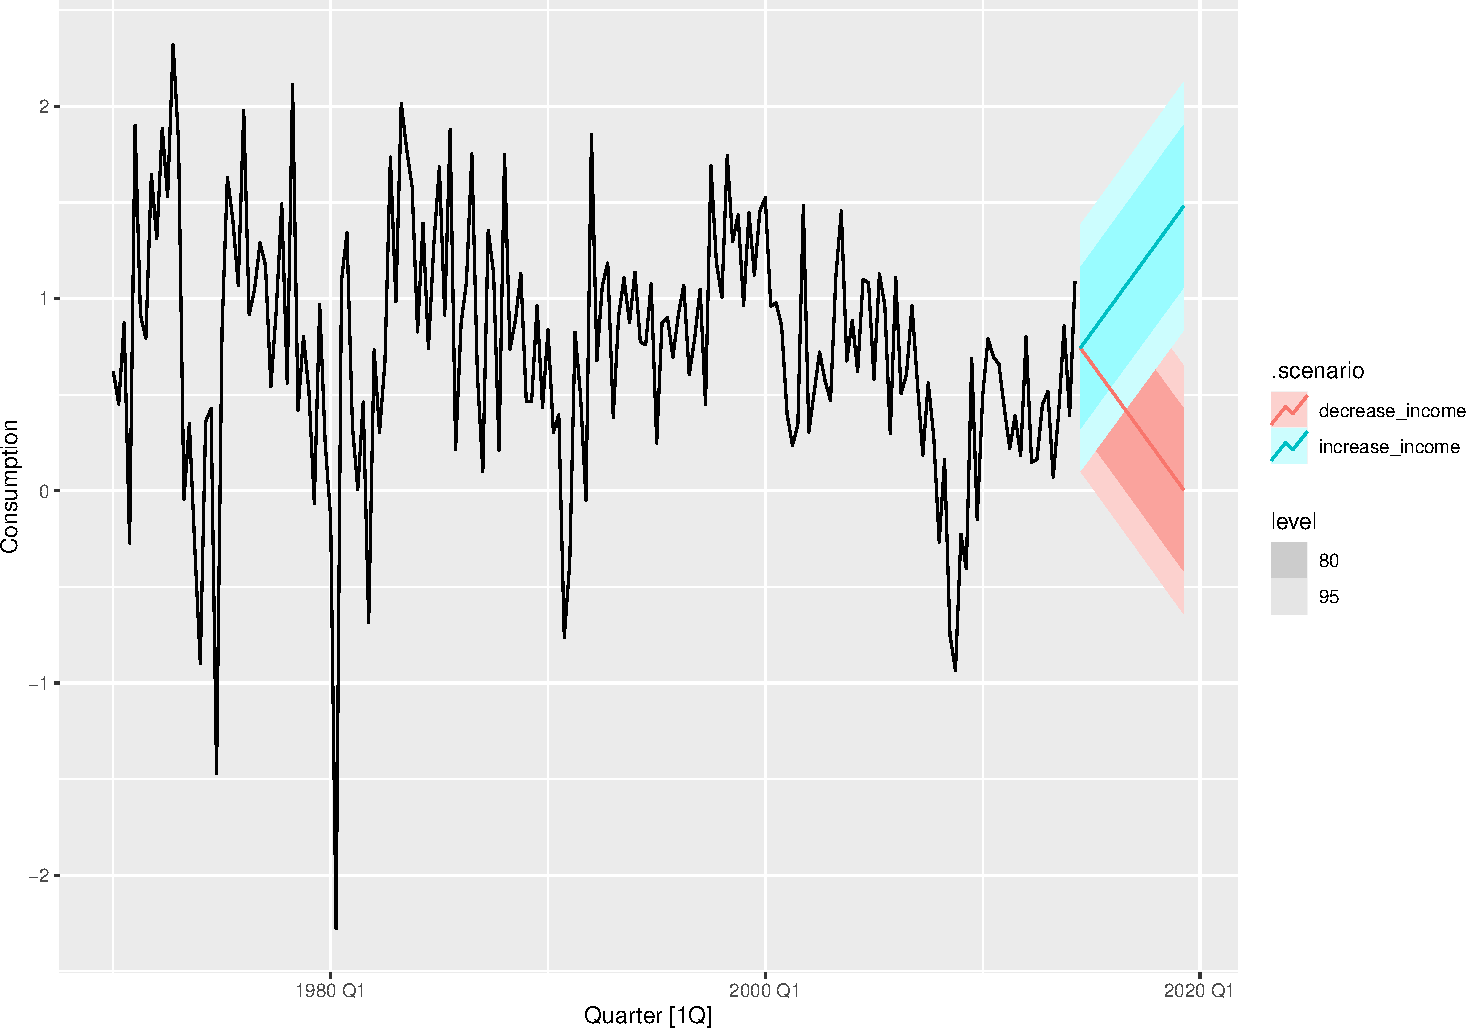
\includegraphics{Time-series-regression-models_files/figure-beamer/unnamed-chunk-31-1.pdf}

\normalfont
\end{frame}

\begin{frame}{Forecasting \textbar{} \small Regression Components}
\protect\hypertarget{forecasting-regression-components}{}
\center Regression with Trend and Seasonal Components
\end{frame}

\begin{frame}{Forecasting \textbar{} \small Regression Components}
\protect\hypertarget{forecasting-regression-components-1}{}
\begin{figure}
\begin{equation*}
\tikzmarknode{y}{\highlight{red}{$y_t$}} =
\tikzmarknode{intercept}{\highlight{skyblue}{$\beta_0$}} +
\tikzmarknode{trend}{\highlight{green}{$\beta_1 t$}} +
\tikzmarknode{error}{\highlight{orange}{$\epsilon_t$}}
\end{equation*}

\begin{tikzpicture}[overlay,remember picture,>=stealth,nodes={align=center,inner ysep=1pt},<-]
    
    % y
    \path (y.north) ++ (0,1em) node[anchor=south east,color=red] (scalep){\textbf{outcome (at time \textit{t})}};
    \draw [color=red](y.north) |- ([xshift=-0.3ex,color=red]scalep.south west);
    
    % intercept
    \path (intercept.south) ++ (0,-1em) node[anchor=north east,color=skyblue] (scalep){\textbf{intercept}};
    \draw [color=skyblue](intercept.south) |- ([xshift=-0.3ex,color=skyblue]scalep.north west);
    
    % trend
    \path (trend.north) ++ (0,1em) node[anchor=south west,color=green] (scalep){\textbf{trend}};
    \draw [color=green](trend.north) |- ([xshift=-0.3ex,color=green]scalep.south east);
    
    % error
    \path (error.south) ++ (0,-1em) node[anchor=north west,color=orange] (scalep){\textbf{error (at time \textit{t})}};
    \draw [color=orange](error.south) |- ([xshift=-0.3ex,color=orange]scalep.north east);
    
\end{tikzpicture}
\vspace{-1.1cm}
\label{fig:fig3}
\end{figure}
\end{frame}

\begin{frame}[fragile]{Forecasting \textbar{} \small Regression Trend
Example}
\protect\hypertarget{forecasting-regression-trend-example}{}
\normalfont

\begin{Shaded}
\begin{Highlighting}[]
\CommentTok{\# Fit linear model with trend}
\NormalTok{  fit\_us\_trend }\OtherTok{\textless{}{-}}\NormalTok{ us\_prediction }\SpecialCharTok{\%\textgreater{}\%}
  \FunctionTok{model}\NormalTok{( }\CommentTok{\# model for time series}
    \AttributeTok{tslm =} \FunctionTok{TSLM}\NormalTok{( }\CommentTok{\# time series linear model}
\NormalTok{      Consumption }\SpecialCharTok{\textasciitilde{}} \FunctionTok{trend}\NormalTok{() }\CommentTok{\# trend component}
\NormalTok{    )}
\NormalTok{  )}
\end{Highlighting}
\end{Shaded}

\normalfont
\end{frame}

\begin{frame}[fragile]{Forecasting \textbar{} \small Regression Trend
Example}
\protect\hypertarget{forecasting-regression-trend-example-1}{}
\footnotesize

\normalfont

\footnotesize

\begin{Shaded}
\begin{Highlighting}[]
\CommentTok{\# Report fit}
\FunctionTok{report}\NormalTok{(fit\_us\_trend)}
\end{Highlighting}
\end{Shaded}

\begin{verbatim}
Series: Consumption 
Model: TSLM 

Residuals:
    Min      1Q  Median      3Q     Max 
-3.1258 -0.3403  0.0366  0.3867  1.4053 

Coefficients:
              Estimate Std. Error t value Pr(>|t|)    
(Intercept)  0.9408053  0.0992577   9.478   <2e-16 ***
trend()     -0.0022103  0.0009618  -2.298   0.0227 *  
---
Signif. codes:  0 '***' 0.001 '**' 0.01 '*' 0.05 '.' 0.1 ' ' 1

Residual standard error: 0.6593 on 176 degrees of freedom
Multiple R-squared: 0.02913,    Adjusted R-squared: 0.02362
F-statistic: 5.281 on 1 and 176 DF, p-value: 0.022733
\end{verbatim}

\normalfont
\end{frame}

\begin{frame}{Forecasting \textbar{} \small Regression Trend Example}
\protect\hypertarget{forecasting-regression-trend-example-2}{}
\footnotesize

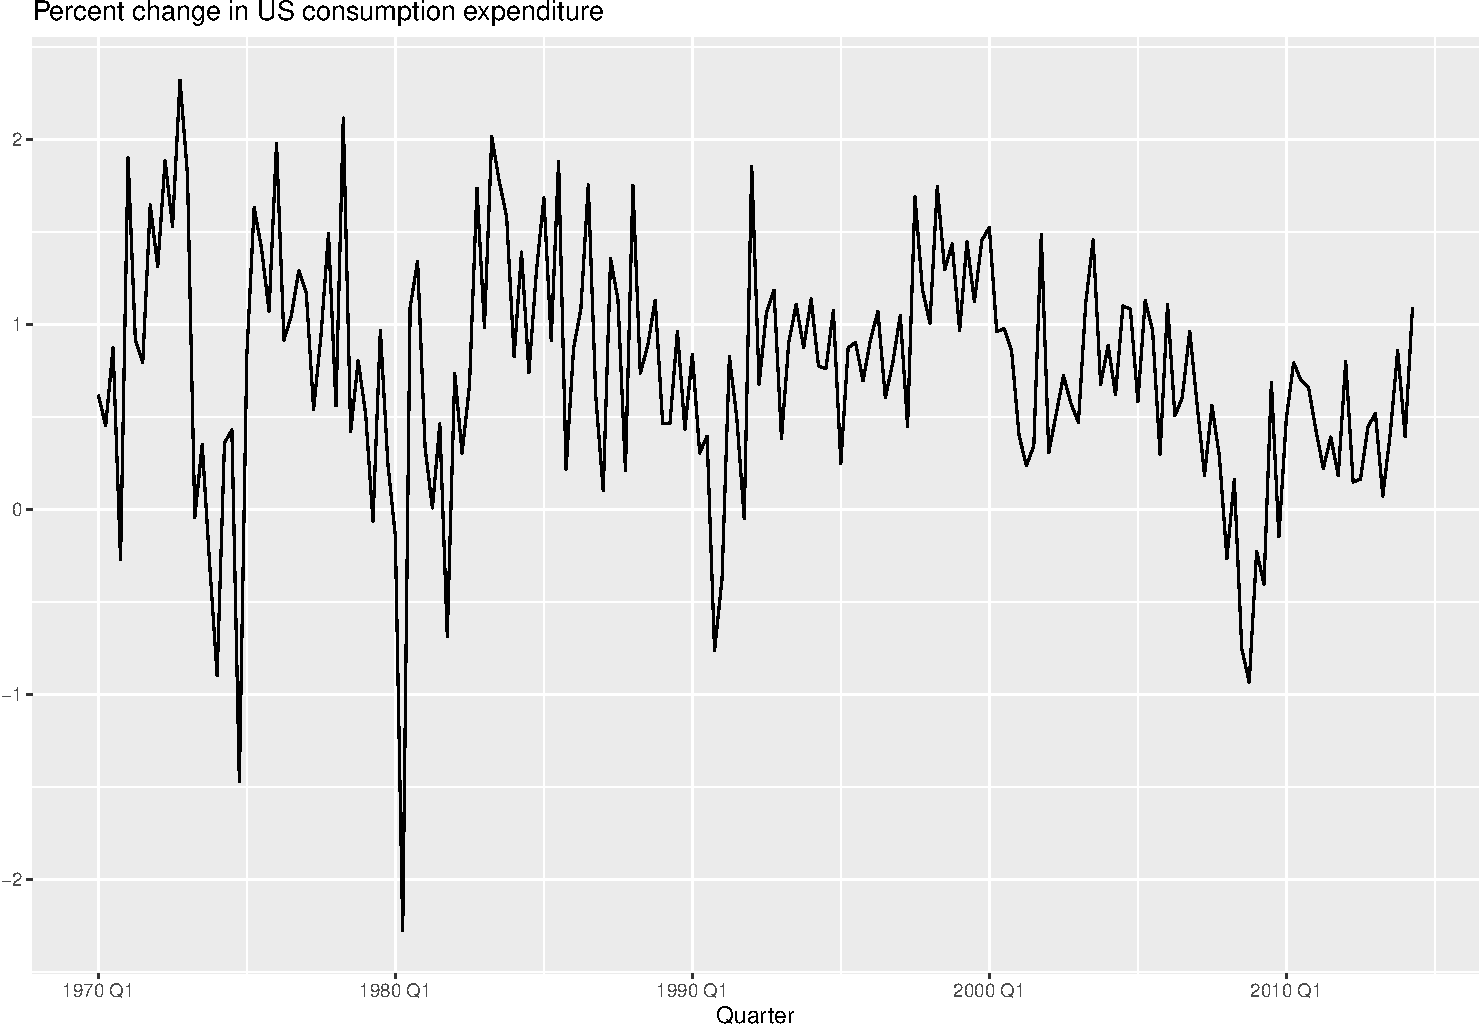
\includegraphics{Time-series-regression-models_files/figure-beamer/unnamed-chunk-35-1.pdf}

\normalfont
\end{frame}

\begin{frame}{Forecasting \textbar{} \small Regression Trend Example}
\protect\hypertarget{forecasting-regression-trend-example-3}{}
\footnotesize

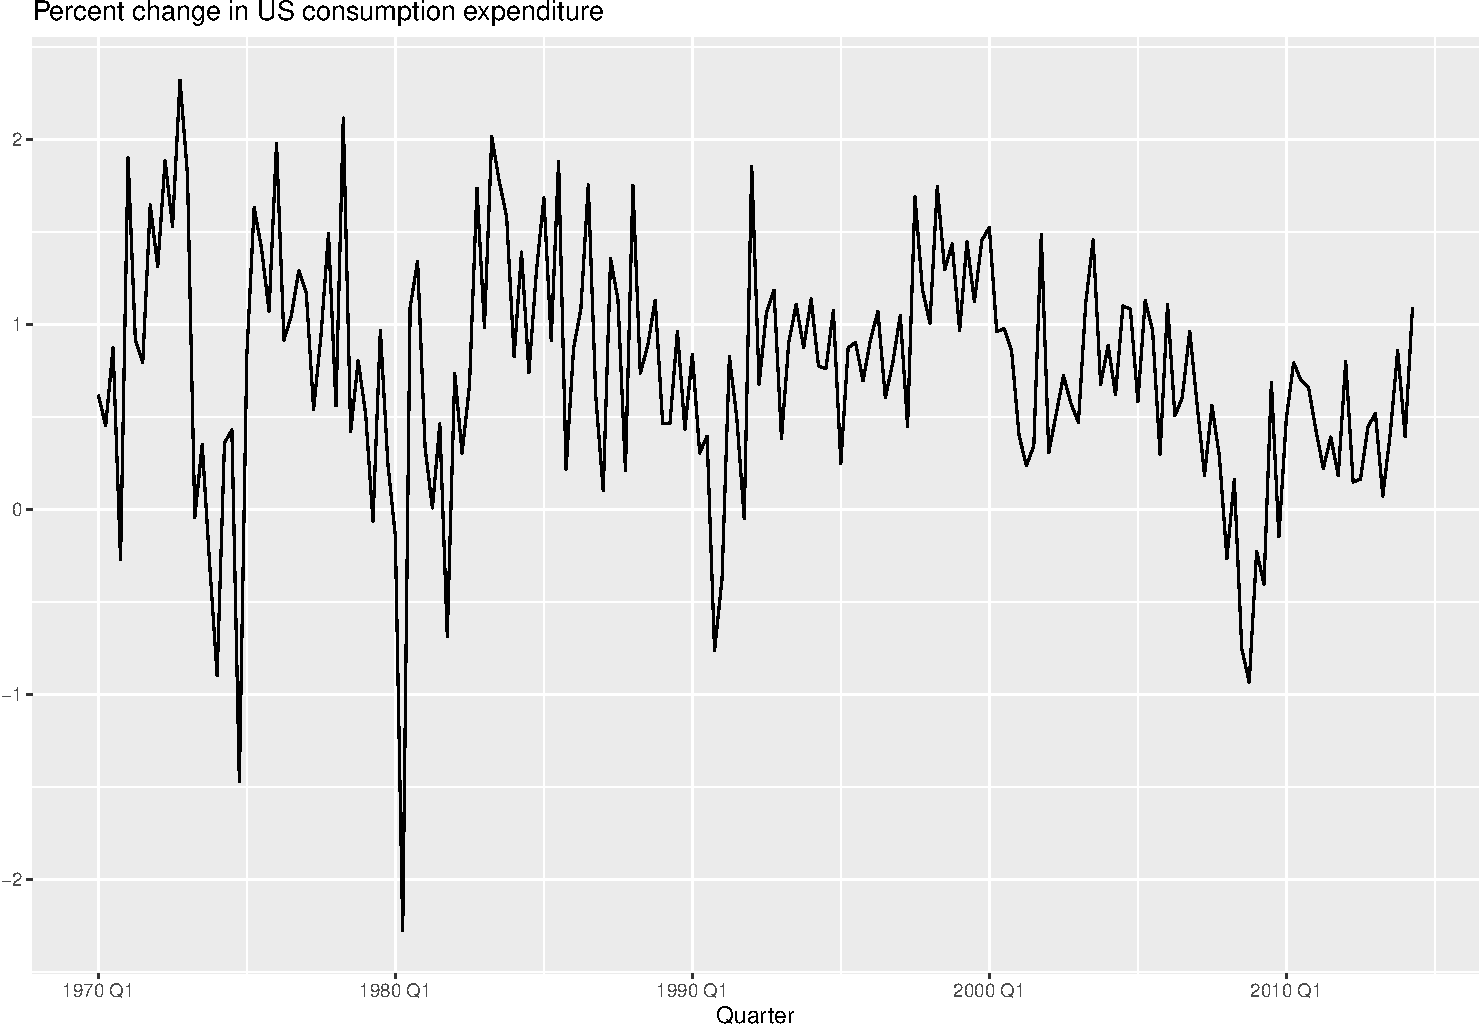
\includegraphics{Time-series-regression-models_files/figure-beamer/unnamed-chunk-36-1.pdf}

\normalfont
\end{frame}

\begin{frame}{Forecasting \textbar{} \small Regression Components}
\protect\hypertarget{forecasting-regression-components-2}{}
\begin{figure}
\begin{equation*}
\tikzmarknode{y}{\highlight{red}{$y_t$}} =
\tikzmarknode{intercept}{\highlight{skyblue}{$\beta_0$}} +
\tikzmarknode{trend}{\highlight{green}{$\beta_1 t$}} +
\tikzmarknode{season}{\highlight{purple}{$\beta_2 d_{2,t} + \beta_3 d_{3,t} + \beta_4 d_{4,t}$}} +
\tikzmarknode{error}{\highlight{orange}{$\epsilon_t$}}
\end{equation*}

\begin{tikzpicture}[overlay,remember picture,>=stealth,nodes={align=center,inner ysep=1pt},<-]
    
    % y
    \path (y.north) ++ (0,1em) node[anchor=south west,color=red] (scalep){\textbf{outcome (at time \textit{t})}};
    \draw [color=red](y.north) |- ([xshift=-0.3ex,color=red]scalep.south east);
    
    % intercept
    \path (intercept.south) ++ (0,-1em) node[anchor=north east,color=skyblue] (scalep){\textbf{intercept}};
    \draw [color=skyblue](intercept.south) |- ([xshift=-0.3ex,color=skyblue]scalep.north west);
    
    % trend
    \path (trend.south) ++ (0,-1em) node[anchor=north west,color=green] (scalep){\textbf{trend}};
    \draw [color=green](trend.south) |- ([xshift=-0.3ex,color=green]scalep.north east);
    
    % season
    \path (season.south) ++ (0,-1em) node[anchor=north west,color=purple] (scalep){\textbf{season}};
    \draw [color=purple](season.south) |- ([xshift=-0.3ex,color=purple]scalep.north east);
    
    % error
    \path (error.south) ++ (0,-1em) node[anchor=north west,color=orange] (scalep){\textbf{error (at time \textit{t})}};
    \draw [color=orange](error.south) |- ([xshift=-0.3ex,color=orange]scalep.north east);
    
\end{tikzpicture}
\vspace{-1.1cm}
\label{fig:fig4}
\end{figure}

\vspace{1cm}

\pause

\begin{table}
\centering
\begin{tabular}{c c c c}

\toprule

 & \(\displaystyle d_{2,t} \) & \(\displaystyle d_{3,t} \) & \(\displaystyle d_{4,t} \) \\ \midrule

Quarter 1 & 0 & 0 & 0 \\

Quarter 2 & 1 & 0 & 0 \\

Quarter 3 & 0 & 1 & 0 \\

Quarter 4 & 0 & 0 & 1 \\

Quarter 1 & 0 & 0 & 0 \\

... & ... & ... & ... \\

\bottomrule

\end{tabular}
\end{table}
\end{frame}

\begin{frame}[fragile]{Forecasting \textbar{} \small Regression Season
Example}
\protect\hypertarget{forecasting-regression-season-example}{}
\footnotesize

\begin{Shaded}
\begin{Highlighting}[]
\CommentTok{\# Fit linear model with trend and season}
\NormalTok{fit\_us\_season }\OtherTok{\textless{}{-}}\NormalTok{ us\_prediction }\SpecialCharTok{\%\textgreater{}\%}
  \FunctionTok{model}\NormalTok{( }\CommentTok{\# model for time series}
    \AttributeTok{tslm =} \FunctionTok{TSLM}\NormalTok{( }\CommentTok{\# time series linear model}
\NormalTok{      Consumption }\SpecialCharTok{\textasciitilde{}} \FunctionTok{trend}\NormalTok{() }\SpecialCharTok{+} \CommentTok{\# trend component}
        \FunctionTok{season}\NormalTok{() }\CommentTok{\# season component}
\NormalTok{    )}
\NormalTok{  )}
\end{Highlighting}
\end{Shaded}

\normalfont
\end{frame}

\begin{frame}[fragile]{Forecasting \textbar{} \small Regression Season
Example}
\protect\hypertarget{forecasting-regression-season-example-1}{}
\tiny

\normalfont

\tiny

\begin{Shaded}
\begin{Highlighting}[]
\CommentTok{\# Report fit}
\FunctionTok{report}\NormalTok{(fit\_us\_season)}
\end{Highlighting}
\end{Shaded}

\begin{verbatim}
Series: Consumption 
Model: TSLM 

Residuals:
     Min       1Q   Median       3Q      Max 
-3.07488 -0.33612  0.00766  0.41042  1.46950 

Coefficients:
                Estimate Std. Error t value Pr(>|t|)    
(Intercept)    0.9380208  0.1306974   7.177 2.01e-11 ***
trend()       -0.0021995  0.0009645  -2.281   0.0238 *  
season()year2 -0.0485962  0.1393858  -0.349   0.7278    
season()year3  0.1186395  0.1401721   0.846   0.3985    
season()year4 -0.0615712  0.1401754  -0.439   0.6610    
---
Signif. codes:  0 '***' 0.001 '**' 0.01 '*' 0.05 '.' 0.1 ' ' 1

Residual standard error: 0.6611 on 173 degrees of freedom
Multiple R-squared: 0.04045,    Adjusted R-squared: 0.01826
F-statistic: 1.823 on 4 and 173 DF, p-value: 0.12648
\end{verbatim}

\normalfont
\end{frame}

\begin{frame}{Forecasting \textbar{} \small Regression Season Example}
\protect\hypertarget{forecasting-regression-season-example-2}{}
\tiny

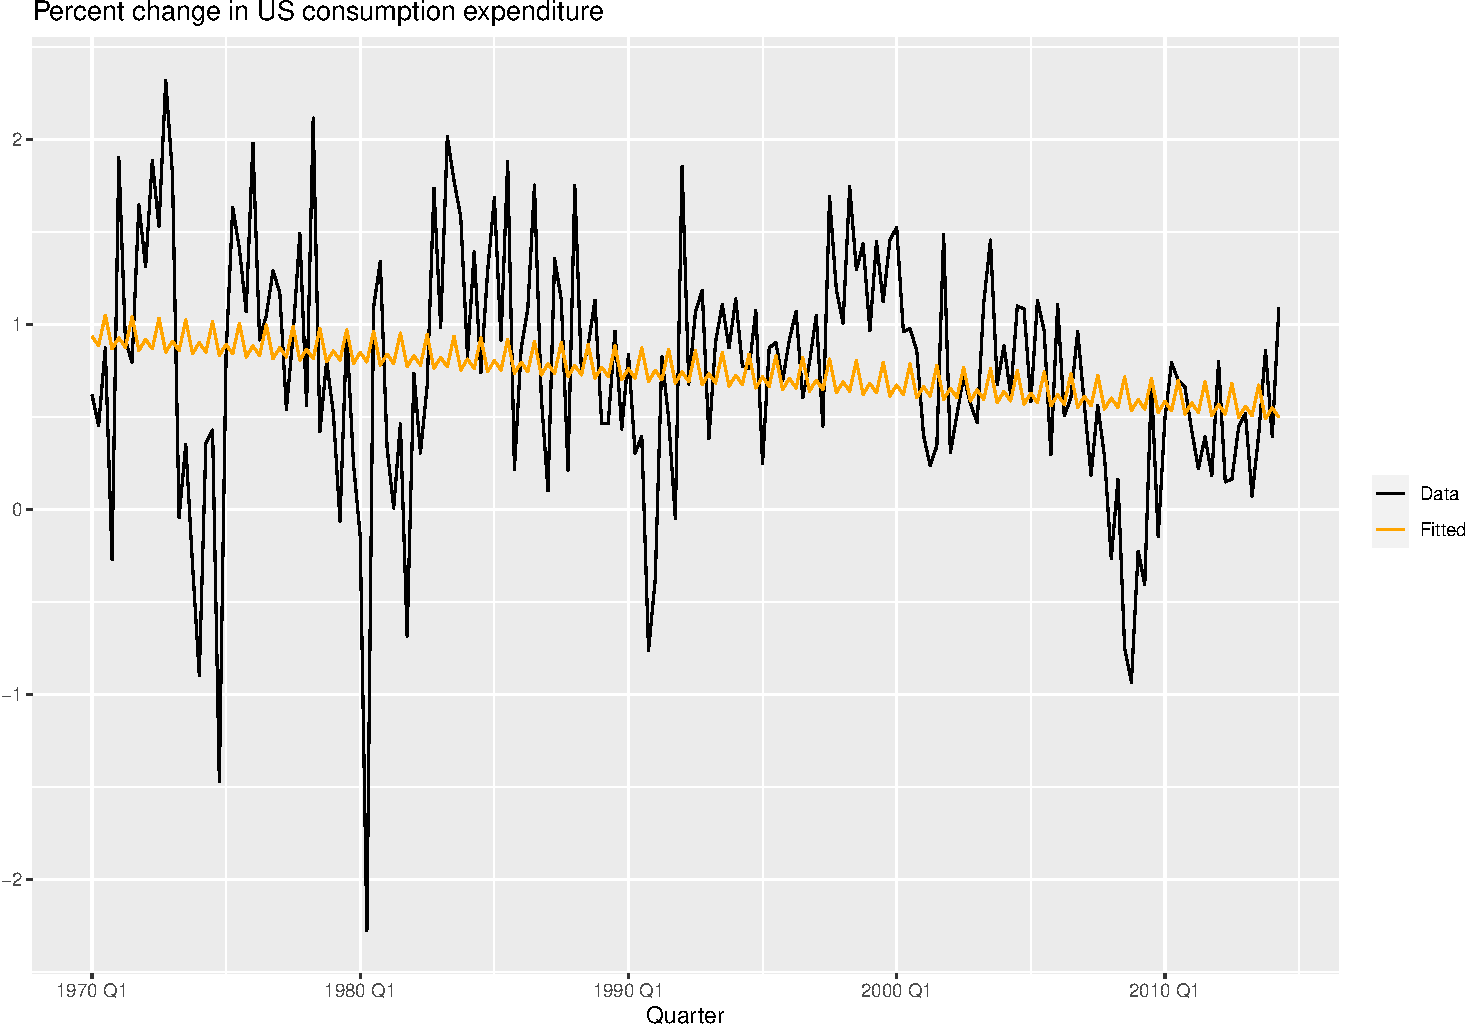
\includegraphics{Time-series-regression-models_files/figure-beamer/unnamed-chunk-40-1.pdf}

\normalfont
\end{frame}

\begin{frame}{Forecasting \textbar{} \small Regression Components}
\protect\hypertarget{forecasting-regression-components-3}{}
\center What happened..?

\pause

\center Let's look at a beer-ter example\ldots{}
\end{frame}

\begin{frame}[fragile]{Forecasting \textbar{} \small A Beer-ter Example}
\protect\hypertarget{forecasting-a-beer-ter-example}{}
\tiny

\begin{Shaded}
\begin{Highlighting}[]
\CommentTok{\# Australian beer production}
\NormalTok{recent\_production }\OtherTok{\textless{}{-}}\NormalTok{ aus\_production }\SpecialCharTok{\%\textgreater{}\%} \FunctionTok{filter}\NormalTok{(}\FunctionTok{year}\NormalTok{(Quarter) }\SpecialCharTok{\textgreater{}=} \DecValTok{1992}\NormalTok{)}
\NormalTok{recent\_production }\SpecialCharTok{\%\textgreater{}\%} \FunctionTok{autoplot}\NormalTok{(Beer) }\SpecialCharTok{+}
  \FunctionTok{labs}\NormalTok{(}\AttributeTok{y=}\StringTok{"Megalitres"}\NormalTok{,}\AttributeTok{title =}\StringTok{"Australian quarterly beer production"}\NormalTok{)}
\end{Highlighting}
\end{Shaded}

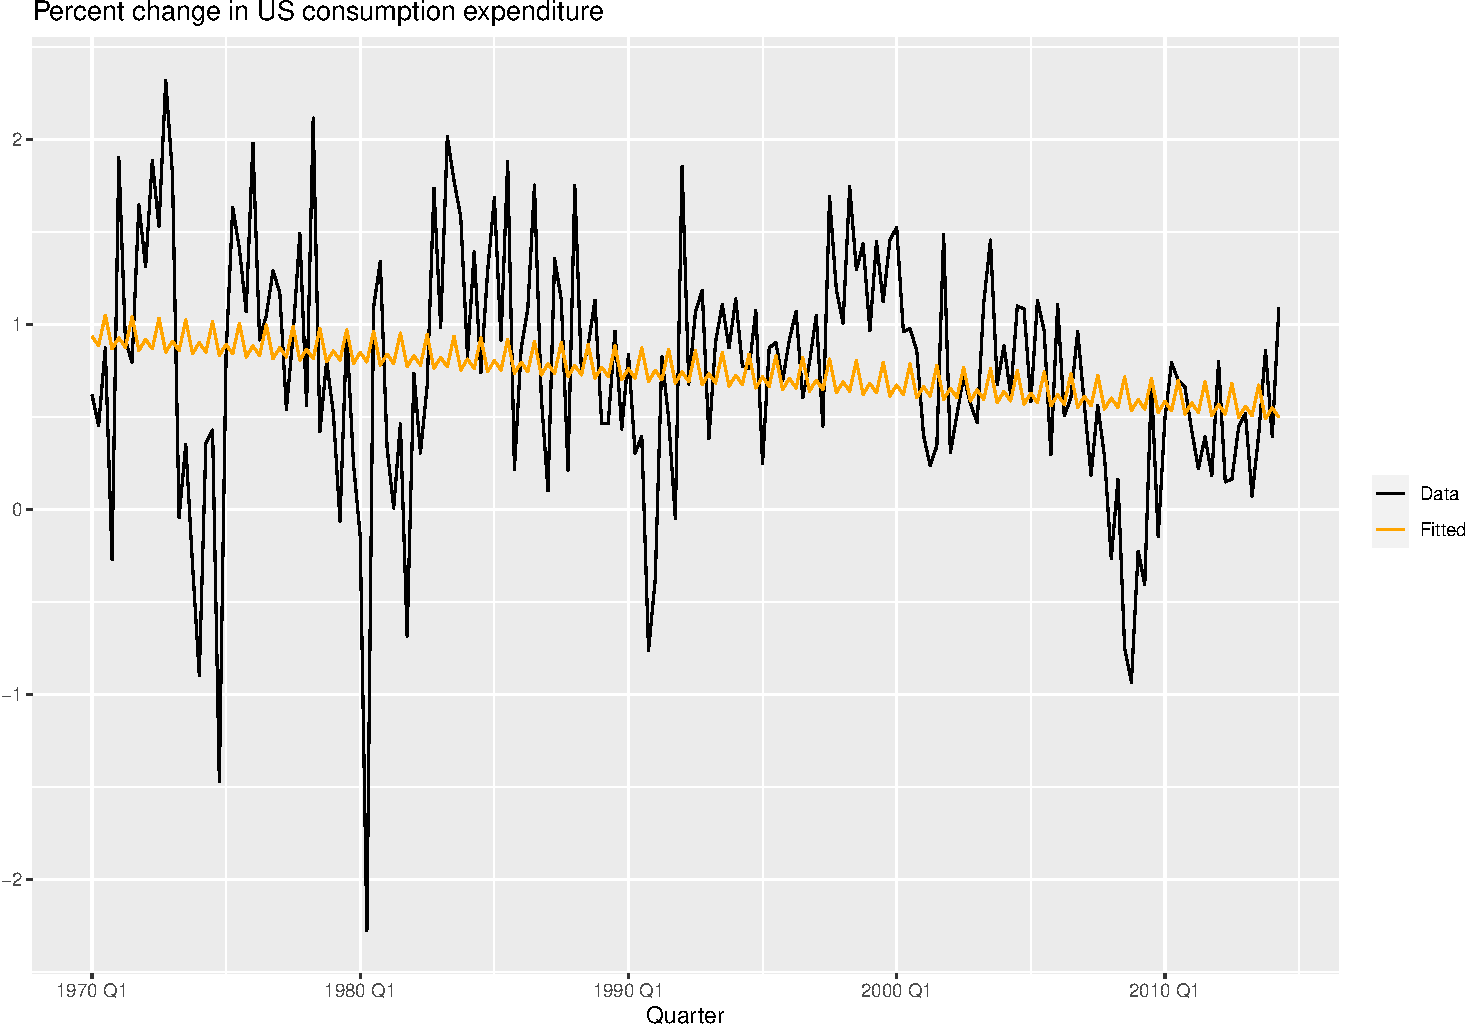
\includegraphics{Time-series-regression-models_files/figure-beamer/unnamed-chunk-41-1.pdf}

\normalfont
\end{frame}

\begin{frame}[fragile]{Forecasting \textbar{} \small A Beer-ter Example}
\protect\hypertarget{forecasting-a-beer-ter-example-1}{}
\tiny

\normalfont

\tiny

\begin{Shaded}
\begin{Highlighting}[]
\CommentTok{\# Fit model}
\NormalTok{fit\_beer }\OtherTok{\textless{}{-}}\NormalTok{ recent\_production }\SpecialCharTok{\%\textgreater{}\%} \FunctionTok{model}\NormalTok{(}\FunctionTok{TSLM}\NormalTok{(Beer }\SpecialCharTok{\textasciitilde{}} \FunctionTok{trend}\NormalTok{() }\SpecialCharTok{+} \FunctionTok{season}\NormalTok{()))}
\NormalTok{fit\_beer }\SpecialCharTok{\%\textgreater{}\%} \FunctionTok{report}\NormalTok{()}
\end{Highlighting}
\end{Shaded}

\begin{verbatim}
Series: Beer 
Model: TSLM 

Residuals:
     Min       1Q   Median       3Q      Max 
-42.9029  -7.5995  -0.4594   7.9908  21.7895 

Coefficients:
               Estimate Std. Error t value Pr(>|t|)    
(Intercept)   441.80044    3.73353 118.333  < 2e-16 ***
trend()        -0.34027    0.06657  -5.111 2.73e-06 ***
season()year2 -34.65973    3.96832  -8.734 9.10e-13 ***
season()year3 -17.82164    4.02249  -4.430 3.45e-05 ***
season()year4  72.79641    4.02305  18.095  < 2e-16 ***
---
Signif. codes:  0 '***' 0.001 '**' 0.01 '*' 0.05 '.' 0.1 ' ' 1

Residual standard error: 12.23 on 69 degrees of freedom
Multiple R-squared: 0.9243, Adjusted R-squared: 0.9199
F-statistic: 210.7 on 4 and 69 DF, p-value: < 2.22e-16
\end{verbatim}

\normalfont
\end{frame}

\begin{frame}[fragile]{Forecasting \textbar{} \small A Beer-ter Example}
\protect\hypertarget{forecasting-a-beer-ter-example-2}{}
\tiny

\begin{Shaded}
\begin{Highlighting}[]
\CommentTok{\# Residuals}
\NormalTok{fit\_beer }\SpecialCharTok{\%\textgreater{}\%}
  \FunctionTok{gg\_tsresiduals}\NormalTok{()}
\end{Highlighting}
\end{Shaded}

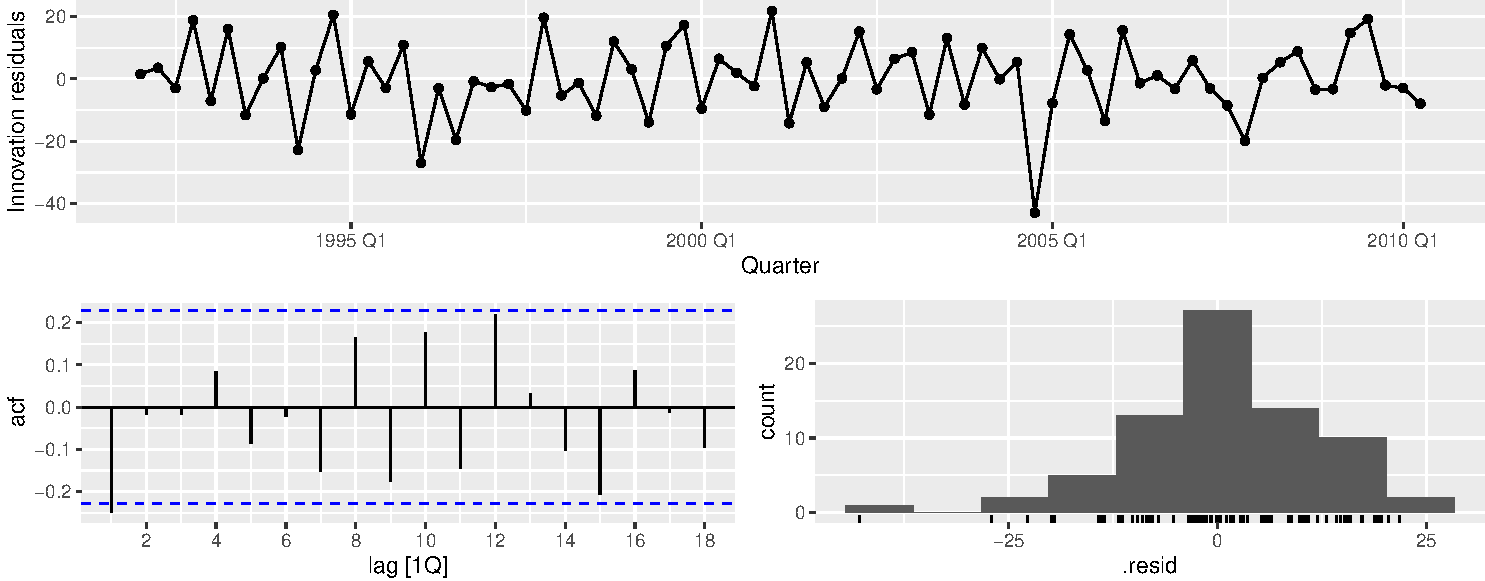
\includegraphics{Time-series-regression-models_files/figure-beamer/unnamed-chunk-44-1.pdf}

\normalfont
\end{frame}

\begin{frame}[fragile]{Forecasting \textbar{} \small A Beer-ter Example}
\protect\hypertarget{forecasting-a-beer-ter-example-3}{}
\tiny

\begin{Shaded}
\begin{Highlighting}[]
\CommentTok{\# Plot fitted model}
\FunctionTok{augment}\NormalTok{(fit\_beer) }\SpecialCharTok{\%\textgreater{}\%}
  \FunctionTok{ggplot}\NormalTok{(}\FunctionTok{aes}\NormalTok{(}\AttributeTok{x =}\NormalTok{ Quarter)) }\SpecialCharTok{+}
  \FunctionTok{geom\_line}\NormalTok{(}\FunctionTok{aes}\NormalTok{(}\AttributeTok{y =}\NormalTok{ Beer, }\AttributeTok{colour =} \StringTok{"Data"}\NormalTok{)) }\SpecialCharTok{+}
  \FunctionTok{geom\_line}\NormalTok{(}\FunctionTok{aes}\NormalTok{(}\AttributeTok{y =}\NormalTok{ .fitted, }\AttributeTok{colour =} \StringTok{"Fitted"}\NormalTok{)) }\SpecialCharTok{+}
  \FunctionTok{labs}\NormalTok{(}\AttributeTok{y=}\StringTok{"Megalitres"}\NormalTok{,}\AttributeTok{title =}\StringTok{"Australian quarterly beer production"}\NormalTok{) }\SpecialCharTok{+}
  \FunctionTok{scale\_colour\_manual}\NormalTok{(}\AttributeTok{values =} \FunctionTok{c}\NormalTok{(}\AttributeTok{Data =} \StringTok{"black"}\NormalTok{, }\AttributeTok{Fitted =} \StringTok{"\#D55E00"}\NormalTok{))}
\end{Highlighting}
\end{Shaded}

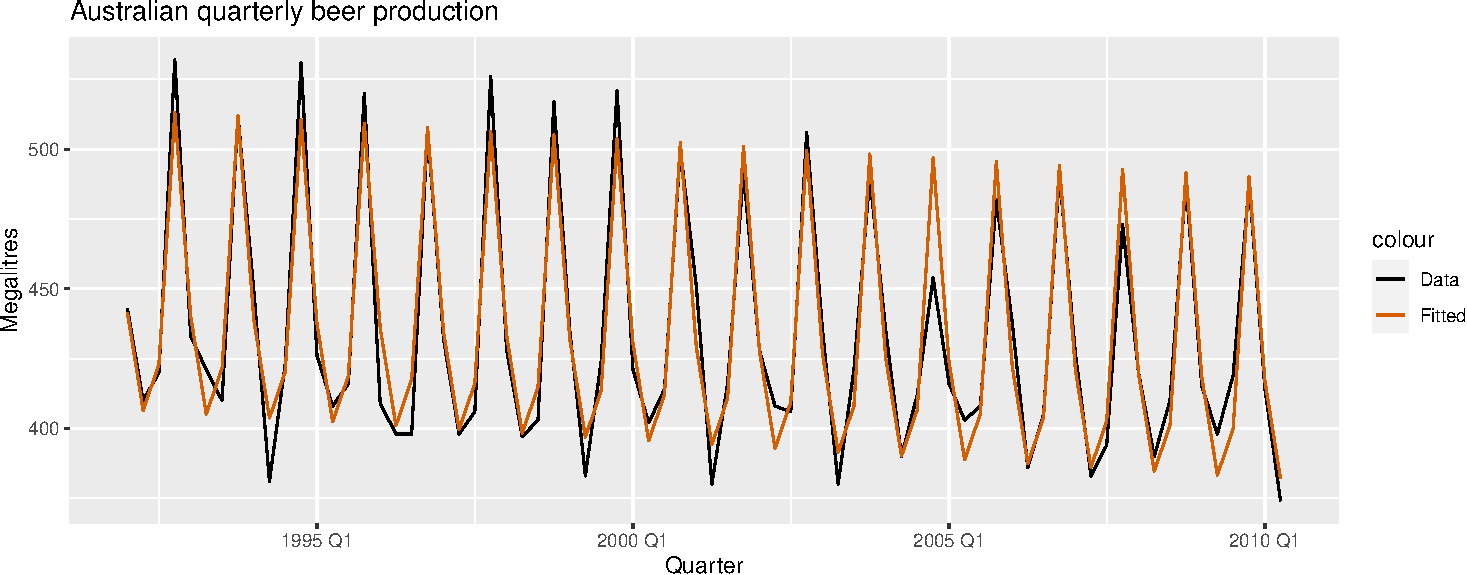
\includegraphics{Time-series-regression-models_files/figure-beamer/unnamed-chunk-45-1.pdf}

\normalfont
\end{frame}

\begin{frame}[fragile]{Forecasting \textbar{} \small A Beer-ter Example}
\protect\hypertarget{forecasting-a-beer-ter-example-4}{}
\tiny

\begin{Shaded}
\begin{Highlighting}[]
\CommentTok{\# Examining seasonality}
\FunctionTok{augment}\NormalTok{(fit\_beer) }\SpecialCharTok{\%\textgreater{}\%}
  \FunctionTok{ggplot}\NormalTok{(}\FunctionTok{aes}\NormalTok{(}\AttributeTok{x=}\NormalTok{Beer, }\AttributeTok{y=}\NormalTok{.fitted, }\AttributeTok{colour=}\FunctionTok{factor}\NormalTok{(}\FunctionTok{quarter}\NormalTok{(Quarter)))) }\SpecialCharTok{+}
    \FunctionTok{geom\_point}\NormalTok{() }\SpecialCharTok{+}
    \FunctionTok{labs}\NormalTok{(}\AttributeTok{y=}\StringTok{"Fitted"}\NormalTok{, }\AttributeTok{x=}\StringTok{"Actual values"}\NormalTok{, }\AttributeTok{title =} \StringTok{"Quarterly beer production"}\NormalTok{) }\SpecialCharTok{+}
    \FunctionTok{scale\_colour\_brewer}\NormalTok{(}\AttributeTok{palette=}\StringTok{"Dark2"}\NormalTok{, }\AttributeTok{name=}\StringTok{"Quarter"}\NormalTok{) }\SpecialCharTok{+}
    \FunctionTok{geom\_abline}\NormalTok{(}\AttributeTok{intercept=}\DecValTok{0}\NormalTok{, }\AttributeTok{slope=}\DecValTok{1}\NormalTok{)}
\end{Highlighting}
\end{Shaded}

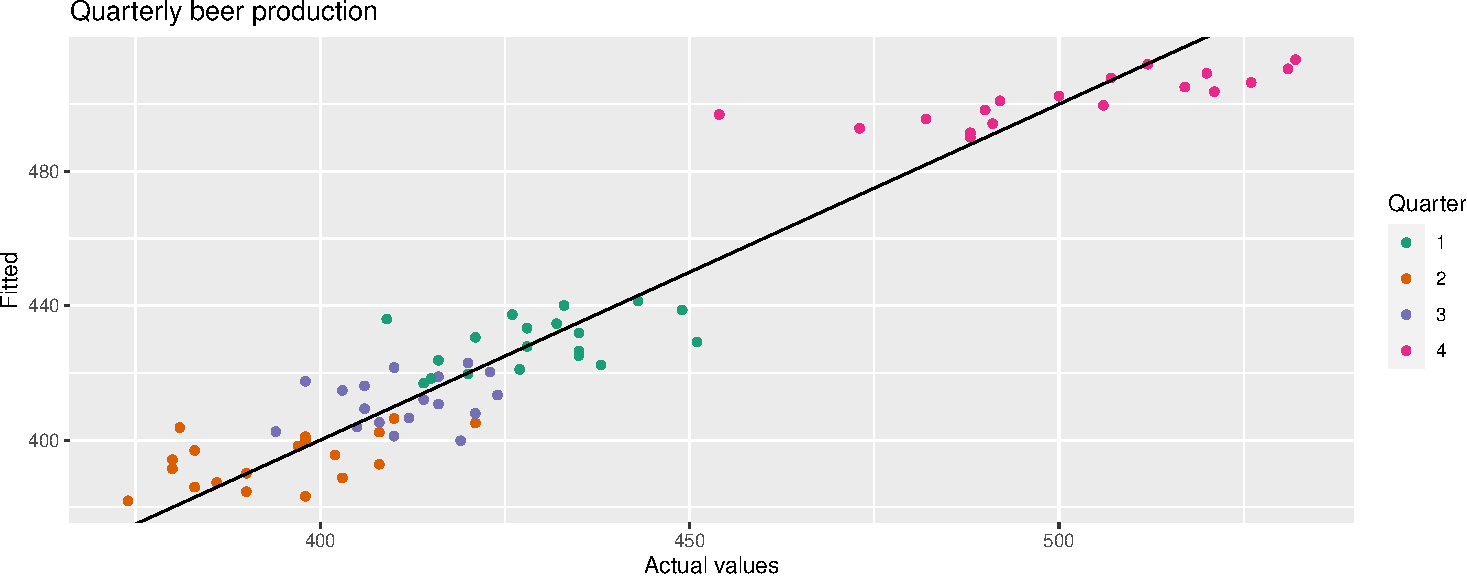
\includegraphics{Time-series-regression-models_files/figure-beamer/unnamed-chunk-46-1.pdf}

\normalfont
\end{frame}

\begin{frame}[fragile]{Forecasting \textbar{} \small A Beer-ter Example}
\protect\hypertarget{forecasting-a-beer-ter-example-5}{}
\tiny

\begin{Shaded}
\begin{Highlighting}[]
\CommentTok{\# Forecasting prediction}
\NormalTok{fc }\OtherTok{\textless{}{-}}\NormalTok{ fit\_beer }\SpecialCharTok{\%\textgreater{}\%}\NormalTok{ forecast}
\CommentTok{\# Plot forecast}
\NormalTok{fc }\SpecialCharTok{\%\textgreater{}\%} \FunctionTok{autoplot}\NormalTok{(recent\_production)}
\end{Highlighting}
\end{Shaded}

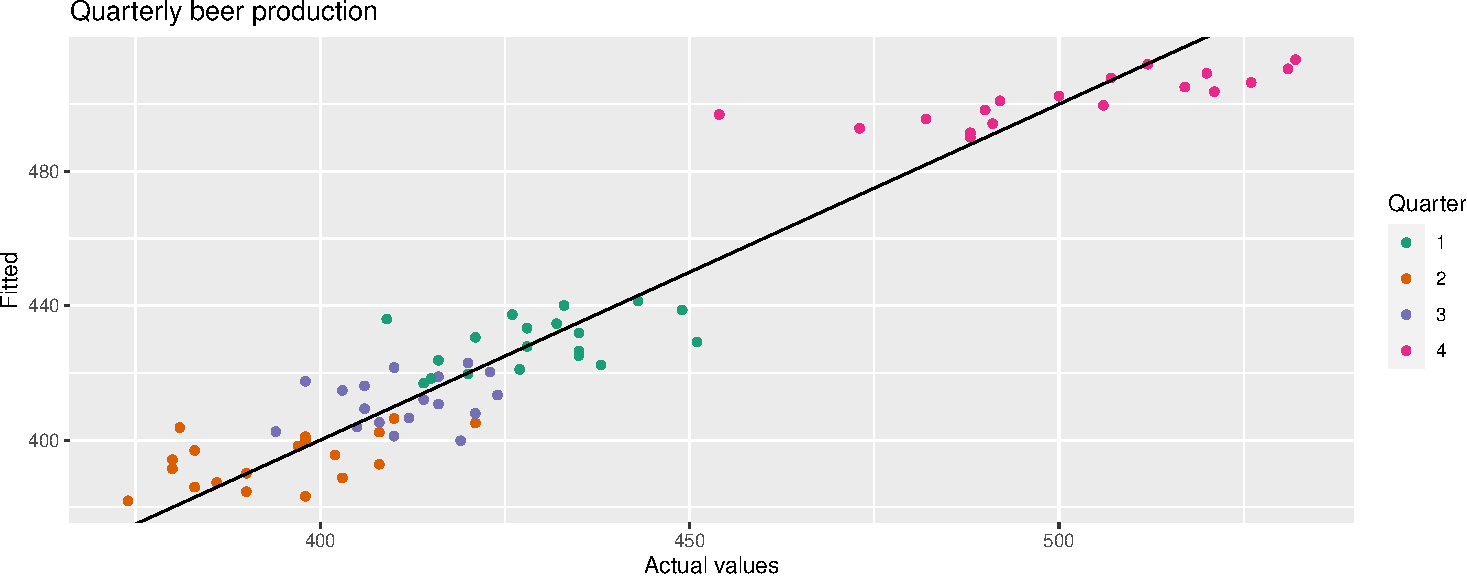
\includegraphics{Time-series-regression-models_files/figure-beamer/unnamed-chunk-47-1.pdf}

\normalfont
\end{frame}

\begin{frame}{Forecasting \textbar{} \small Regression Fit}
\protect\hypertarget{forecasting-regression-fit}{}
\begin{block}{Measures of Fit}
\protect\hypertarget{measures-of-fit}{}
\begin{itemize}
\tightlist
\item
  Adjusted R-squared: proportion of variance explained \newline
\end{itemize}

\center \(\bar{R^2} = 1 - (1 - R^2) \frac{T - 1}{T - k - 1}\) \newline

\begin{itemize}
\tightlist
\item
  Cross-validation: \newline
\end{itemize}

\begin{enumerate}
\item
  Remove time point \(t\), fit model, and compute error
  \(e^*_t = y_t - \hat{y_t}\) \newline
\item
  Repeat for each time point \(T\) \newline
\item
  Compute MSE
\end{enumerate}

\center \(MSE = \frac{\sum (\hat{y_t} - y_t)^2}{T}\) \newline
\end{block}
\end{frame}

\begin{frame}{Forecasting \textbar{} \small Regression Fit}
\protect\hypertarget{forecasting-regression-fit-1}{}
\begin{block}{Measures of Fit}
\protect\hypertarget{measures-of-fit-1}{}
\begin{itemize}
\tightlist
\item
  Akaike's Information Criterion \newline
\end{itemize}

\center \(AIC = T \log \bigg(\frac{SSE}{T}\bigg) + 2(k+2)\) \newline

\center \(SSE = \sum_{t=1}^T e^2_t\) \newline

\begin{itemize}
\tightlist
\item
  Corrected Akaike's Information Criterion \newline
\end{itemize}

\center \(AIC_c = AIC + \frac{2(k+2)(k+3)}{T - k - 3}\) \newline

\begin{itemize}
\tightlist
\item
  Schwarz's Bayesian Information Criterion \newline
\end{itemize}

\center \(BIC = T \log \bigg(\frac{SSE}{T}\bigg) + (k+2) \log(T)\)
\end{block}
\end{frame}

\begin{frame}[fragile]{Forecasting \textbar{} \small Regression Fit}
\protect\hypertarget{forecasting-regression-fit-2}{}
\footnotesize

\normalfont

\footnotesize

\begin{Shaded}
\begin{Highlighting}[]
\CommentTok{\# Report fit measures}
\FunctionTok{glance}\NormalTok{(fit\_beer) }\SpecialCharTok{\%\textgreater{}\%}
  \FunctionTok{select}\NormalTok{(}
\NormalTok{    adj\_r\_squared, CV, AIC, AICc, BIC}
\NormalTok{  )}
\end{Highlighting}
\end{Shaded}

\begin{verbatim}
# A tibble: 1 x 5
  adj_r_squared    CV   AIC  AICc   BIC
          <dbl> <dbl> <dbl> <dbl> <dbl>
1         0.920  160.  377.  379.  391.
\end{verbatim}

\normalfont
\end{frame}

\begin{frame}{Forecasting \textbar{} \small Regression Considerations}
\protect\hypertarget{forecasting-regression-considerations}{}
Dummy Variables

\begin{small}

+ Interventions (one time): An effect that lasts only one period. Add a dummy variable with 1 at time point ($t$)

+ Interventions (permanent): An effect that continues. Add a dummy variable with 1 at time point ($t$) and each time point there after ($t, t_{+1}, ..., t_n$)

+ Number of days: Use number of days in each month as a regressor

+ Lags: Inclusion of previous time points to predict current time point

+ Holidays: Adjust placement of 1 with each year

+ Fourier series (alternative to season): sine and cosine based on $m$ periods (e.g., $m = 52$ for weeks in a year)

\end{small}
\end{frame}

\begin{frame}{Forecasting \textbar{} \small Fourier Series}
\protect\hypertarget{forecasting-fourier-series}{}
\center Fourier Example
\end{frame}

\begin{frame}[fragile]{Forecasting \textbar{} \small Fourier Series}
\protect\hypertarget{forecasting-fourier-series-1}{}
Periodic seasonality can be handled using pairs of Fourier terms

\[
s_{k}(t) = \sin\left(\frac{2\pi k t}{m}\right)\qquad c_{k}(t) = \cos\left(\frac{2\pi k t}{m}\right)
\] \[
y_t = a + bt + \sum_{k=1}^K \left[\alpha_k s_k(t) + \beta_k c_k(t)\right] + \varepsilon_t
\]

\begin{itemize}
\item
  Every periodic function can be approximated by sums of sin and cos
  terms for large enough \(K\).
\item
  Choose \(K\) by minimizing AICc
\item
  Called ``harmonic regression''
\end{itemize}

\footnotesize

\begin{Shaded}
\begin{Highlighting}[]
\FunctionTok{TSLM}\NormalTok{(y }\SpecialCharTok{\textasciitilde{}} \FunctionTok{trend}\NormalTok{() }\SpecialCharTok{+} \FunctionTok{fourier}\NormalTok{(K))}
\end{Highlighting}
\end{Shaded}

\normalfont
\end{frame}

\begin{frame}[fragile]{Forecasting \textbar{} \small Fourier Series}
\protect\hypertarget{forecasting-fourier-series-2}{}
\tiny

\normalfont

\tiny

\begin{Shaded}
\begin{Highlighting}[]
\CommentTok{\# Harmonic regression}
\NormalTok{fourier\_beer }\OtherTok{\textless{}{-}}\NormalTok{ recent\_production }\SpecialCharTok{\%\textgreater{}\%}
  \FunctionTok{model}\NormalTok{( }\CommentTok{\# model for time series}
    \AttributeTok{tslm =} \FunctionTok{TSLM}\NormalTok{( }\CommentTok{\# time series linear model}
\NormalTok{      Beer }\SpecialCharTok{\textasciitilde{}} \FunctionTok{trend}\NormalTok{() }\SpecialCharTok{+} \CommentTok{\# trend component}
        \FunctionTok{fourier}\NormalTok{(}\AttributeTok{K =} \DecValTok{2}\NormalTok{) }\CommentTok{\# harmonic regression}
\NormalTok{    )}
\NormalTok{  )}

\CommentTok{\# Report fit}
\FunctionTok{report}\NormalTok{(fourier\_beer)}
\end{Highlighting}
\end{Shaded}

\begin{verbatim}
Series: Beer 
Model: TSLM 

Residuals:
     Min       1Q   Median       3Q      Max 
-42.9029  -7.5995  -0.4594   7.9908  21.7895 

Coefficients:
                    Estimate Std. Error t value Pr(>|t|)    
(Intercept)        446.87920    2.87321 155.533  < 2e-16 ***
trend()             -0.34027    0.06657  -5.111 2.73e-06 ***
fourier(K = 2)C1_4   8.91082    2.01125   4.430 3.45e-05 ***
fourier(K = 2)S1_4 -53.72807    2.01125 -26.714  < 2e-16 ***
fourier(K = 2)C2_4 -13.98958    1.42256  -9.834 9.26e-15 ***
---
Signif. codes:  0 '***' 0.001 '**' 0.01 '*' 0.05 '.' 0.1 ' ' 1

Residual standard error: 12.23 on 69 degrees of freedom
Multiple R-squared: 0.9243, Adjusted R-squared: 0.9199
F-statistic: 210.7 on 4 and 69 DF, p-value: < 2.22e-16
\end{verbatim}

\normalfont
\end{frame}

\begin{frame}[fragile]{Forecasting \textbar{} \small Fourier Series}
\protect\hypertarget{forecasting-fourier-series-3}{}
Selecting a model:

\tiny

\begin{Shaded}
\begin{Highlighting}[]
\CommentTok{\# Fit multiple models}
\NormalTok{fit }\OtherTok{\textless{}{-}}\NormalTok{ recent\_production }\SpecialCharTok{\%\textgreater{}\%}
  \FunctionTok{model}\NormalTok{(}
    \AttributeTok{K1 =} \FunctionTok{TSLM}\NormalTok{(Beer }\SpecialCharTok{\textasciitilde{}} \FunctionTok{trend}\NormalTok{() }\SpecialCharTok{+} \FunctionTok{fourier}\NormalTok{(}\AttributeTok{K =} \DecValTok{1}\NormalTok{)),}
    \AttributeTok{K2 =} \FunctionTok{TSLM}\NormalTok{(Beer }\SpecialCharTok{\textasciitilde{}} \FunctionTok{trend}\NormalTok{() }\SpecialCharTok{+} \FunctionTok{fourier}\NormalTok{(}\AttributeTok{K =} \DecValTok{2}\NormalTok{)),}
    \AttributeTok{K3 =} \FunctionTok{TSLM}\NormalTok{(Beer }\SpecialCharTok{\textasciitilde{}} \FunctionTok{trend}\NormalTok{() }\SpecialCharTok{+} \FunctionTok{fourier}\NormalTok{(}\AttributeTok{K =} \DecValTok{3}\NormalTok{)),}
    \AttributeTok{K4 =} \FunctionTok{TSLM}\NormalTok{(Beer }\SpecialCharTok{\textasciitilde{}} \FunctionTok{trend}\NormalTok{() }\SpecialCharTok{+} \FunctionTok{fourier}\NormalTok{(}\AttributeTok{K =} \DecValTok{4}\NormalTok{)),}
    \AttributeTok{K5 =} \FunctionTok{TSLM}\NormalTok{(Beer }\SpecialCharTok{\textasciitilde{}} \FunctionTok{trend}\NormalTok{() }\SpecialCharTok{+} \FunctionTok{fourier}\NormalTok{(}\AttributeTok{K =} \DecValTok{5}\NormalTok{)),}
    \AttributeTok{K6 =} \FunctionTok{TSLM}\NormalTok{(Beer }\SpecialCharTok{\textasciitilde{}} \FunctionTok{trend}\NormalTok{() }\SpecialCharTok{+} \FunctionTok{fourier}\NormalTok{(}\AttributeTok{K =} \DecValTok{6}\NormalTok{))}
\NormalTok{  )}

\CommentTok{\# Check fit}
\FunctionTok{glance}\NormalTok{(fit) }\SpecialCharTok{\%\textgreater{}\%} \FunctionTok{select}\NormalTok{(.model, r\_squared, adj\_r\_squared, AICc)}
\end{Highlighting}
\end{Shaded}

\begin{verbatim}
# A tibble: 2 x 4
  .model r_squared adj_r_squared  AICc
  <chr>      <dbl>         <dbl> <dbl>
1 K1         0.818         0.810  441.
2 K2         0.924         0.920  379.
\end{verbatim}

\normalfont
\end{frame}

\begin{frame}[fragile]{Forecasting \textbar{} \small Fourier Series}
\protect\hypertarget{forecasting-fourier-series-4}{}
\tiny

\begin{Shaded}
\begin{Highlighting}[]
\CommentTok{\# Plot fitted model}
\FunctionTok{augment}\NormalTok{(fourier\_beer) }\SpecialCharTok{\%\textgreater{}\%}
  \FunctionTok{ggplot}\NormalTok{(}\FunctionTok{aes}\NormalTok{(}\AttributeTok{x =}\NormalTok{ Quarter)) }\SpecialCharTok{+}
  \FunctionTok{geom\_line}\NormalTok{(}\FunctionTok{aes}\NormalTok{(}\AttributeTok{y =}\NormalTok{ Beer, }\AttributeTok{colour =} \StringTok{"Data"}\NormalTok{)) }\SpecialCharTok{+}
  \FunctionTok{geom\_line}\NormalTok{(}\FunctionTok{aes}\NormalTok{(}\AttributeTok{y =}\NormalTok{ .fitted, }\AttributeTok{colour =} \StringTok{"Fitted"}\NormalTok{)) }\SpecialCharTok{+}
  \FunctionTok{labs}\NormalTok{(}\AttributeTok{y=}\StringTok{"Megalitres"}\NormalTok{,}\AttributeTok{title =}\StringTok{"Australian quarterly beer production"}\NormalTok{) }\SpecialCharTok{+}
  \FunctionTok{scale\_colour\_manual}\NormalTok{(}\AttributeTok{values =} \FunctionTok{c}\NormalTok{(}\AttributeTok{Data =} \StringTok{"black"}\NormalTok{, }\AttributeTok{Fitted =} \StringTok{"\#D55E00"}\NormalTok{))}
\end{Highlighting}
\end{Shaded}

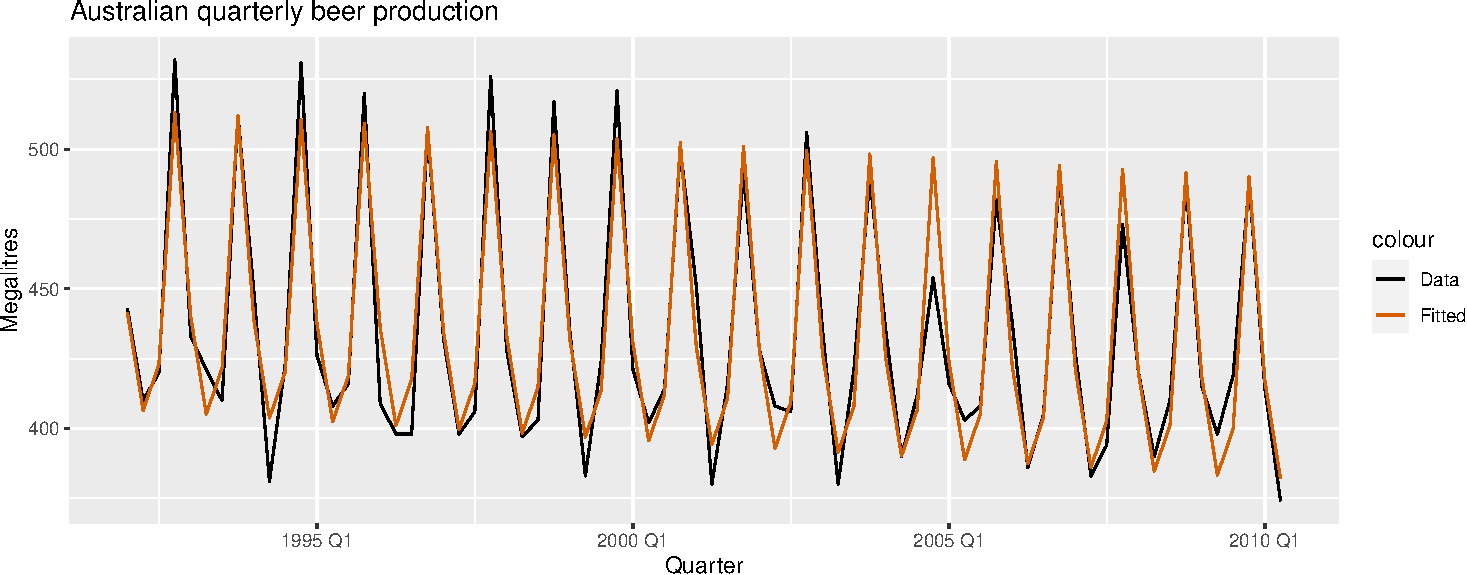
\includegraphics{Time-series-regression-models_files/figure-beamer/unnamed-chunk-54-1.pdf}

\normalfont
\end{frame}

\begin{frame}{Residuals}
\protect\hypertarget{residuals}{}
\center Residual Diagnostics
\end{frame}

\begin{frame}[fragile]{Residuals \textbar{} \small Computing}
\protect\hypertarget{residuals-computing}{}
\tiny

\begin{Shaded}
\begin{Highlighting}[]
\CommentTok{\# Plot fitted model}
\NormalTok{fourier\_beer }\SpecialCharTok{\%\textgreater{}\%}
  \FunctionTok{gg\_tsresiduals}\NormalTok{()}
\end{Highlighting}
\end{Shaded}

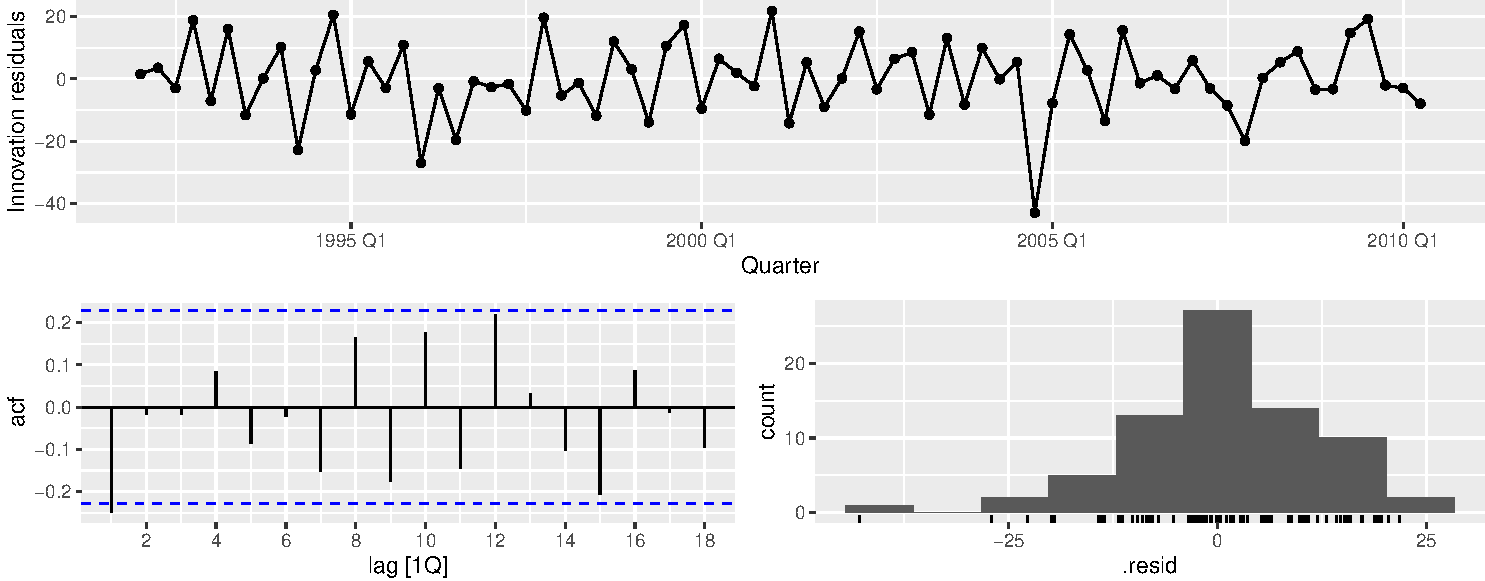
\includegraphics{Time-series-regression-models_files/figure-beamer/unnamed-chunk-55-1.pdf}

\normalfont
\end{frame}

\begin{frame}{Residuals \textbar{} \small Interpreting}
\protect\hypertarget{residuals-interpreting}{}
\begin{itemize}
\item
  \(\epsilon_t\) have zero mean, uncorrelated, and uncorrelated with
  each \(x_{k, t}\)
\item
  Normal distribution (\(\epsilon_t \sim N(0, \sigma^2)\))
  \textbf{useful} for prediction intervals and statistical tests
\item
  If there is a pattern:

  \begin{itemize}
  \tightlist
  \item
    predictor used: possible \textit{nonlinear} relationship between
    residual and predictor
  \item
    predictor \textit{not} used: predictor should be added to model
  \end{itemize}
\end{itemize}
\end{frame}

\begin{frame}{Reading and Homework}
\protect\hypertarget{reading-and-homework}{}
\center Reading and Homework
\end{frame}

\begin{frame}[fragile]{Reading and Homework}
\protect\hypertarget{reading-and-homework-1}{}
\begin{enumerate}
\item
  Read Chapter 7 in FPP3 (7.8 and 7.9 optional) \newline
\item
  Use and complete \texttt{Week2-Homework.Rmd}
\item
  Save file:
  \texttt{{[}LASTNAME{]}\_{[}FIRSTNAME{]}\_Week2-Homework.Rmd}
\item
  Turn in \texttt{.Rmd} or \texttt{HTML} over Brightspace by Sunday
  (04.09.2022)
\end{enumerate}
\end{frame}

\end{document}
